% Classe do documento e parâmetros gerais.
\documentclass[a4paper,openright,twoside,11pt]{report}

% Packages utilizadas e respetivos parâmetros.
\usepackage[utf8]{inputenc}
\usepackage[english]{babel}
\addto{\captionsenglish}{\renewcommand{\bibname}{References}}
\addto{\captionsenglish}{\renewcommand{\contentsname}{Table of Contents}}
\addto{\captionsenglish}{\renewcommand{\appendixname}{Appendix}}

\usepackage{graphicx}
% \texttt break
\usepackage{seqsplit}
\let\originaltexttt\texttt
\renewcommand{\texttt}[1]{%
  \begingroup
    \spaceskip=\fontdimen2\font plus \fontdimen3\font minus \fontdimen4\font
    \originaltexttt{\seqsplit{#1}}%
  \endgroup
}
\usepackage{placeins} % \FloatBarrier: keeps figures from drifting past the
                       % point they're declared, without forcing blank gaps
                       % the way a strict [H] placement would
\usepackage{pdflscape} % rotated, landscape pages for wide appendix figures
\usepackage{url}
\usepackage{tikz}
\usetikzlibrary{shapes.geometric,calc,arrows.meta}
\usepackage[Algoritmo]{algorithm}
\usepackage{algorithmicx}
\usepackage{algpseudocode}
\renewcommand{\algorithmicrequire}{\textbf{Dados: }}
\renewcommand{\algorithmicensure}{\textbf{Resultado: }}

% Código-fonte (listagens numeradas, referenciáveis como figuras)
\usepackage{xcolor}
\usepackage{listings} % numbers listings per chapter automatically in report class
\usepackage{caption}
% Ragged-right only for code listing captions: their unbreakable \texttt{path}
% tokens otherwise get stretched across a justified two-line caption.
\captionsetup[lstlisting]{justification=raggedright, singlelinecheck=false}

\definecolor{codebg}{RGB}{245,245,245}
\definecolor{codekeyword}{RGB}{0,0,180}
\definecolor{codecomment}{RGB}{110,110,110}
\definecolor{codestring}{RGB}{0,120,0}

\lstdefinelanguage{TypeScript}{
    keywords={const, let, var, function, return, if, else, for, while, class,
        interface, type, export, import, from, extends, implements, new, this,
        typeof, async, await, public, private, protected, readonly, enum, as,
        in, of, void, null, undefined, true, false, default, throw, try, catch,
        string, number, boolean, any, unknown, never, satisfies},
    keywordstyle=\color{codekeyword}\bfseries,
    sensitive=true,
    comment=[l]{//},
    morecomment=[s]{/*}{*/},
    commentstyle=\color{codecomment}\itshape,
    string=[b]",
    morestring=[b]',
    morestring=[b]`,
    stringstyle=\color{codestring},
}

\lstset{
    language=TypeScript,
    backgroundcolor=\color{codebg},
    basicstyle=\ttfamily\footnotesize,
    breaklines=true,
    breakatwhitespace=false,
    showstringspaces=false,
    numbers=left,
    numberstyle=\tiny\color{black!50},
    frame=single,
    rulecolor=\color{black!30},
    tabsize=2,
    captionpos=b,
    columns=flexible,
    literate=
        {á}{{\'a}}1 {à}{{\`a}}1 {â}{{\^a}}1 {ã}{{\~a}}1
        {Á}{{\'A}}1 {À}{{\`A}}1 {Â}{{\^A}}1 {Ã}{{\~A}}1
        {é}{{\'e}}1 {ê}{{\^e}}1 {É}{{\'E}}1 {Ê}{{\^E}}1
        {í}{{\'i}}1 {Í}{{\'I}}1
        {ó}{{\'o}}1 {ô}{{\^o}}1 {õ}{{\~o}}1 {Ó}{{\'O}}1 {Ô}{{\^O}}1 {Õ}{{\~O}}1
        {ú}{{\'u}}1 {Ú}{{\'U}}1
        {ç}{{\c c}}1 {Ç}{{\c C}}1,
}

\renewcommand{\lstlistingname}{Listing}
\renewcommand{\lstlistlistingname}{List of Listings}

% Definições das dimensões das páginas
\setlength{\textheight}{24.00cm}
\setlength{\textwidth}{15.50cm}
\setlength{\topmargin}{0.35cm}
\setlength{\headheight}{0cm}
\setlength{\headsep}{0cm}
\setlength{\oddsidemargin}{0.25cm}
\setlength{\evensidemargin}{0.25cm}

%\renewcommand{\baselinestretch}{1}

% Página inicial (capa)
\title{
   \vspace{-50mm}
   \begin{minipage}[l]{\textwidth}
      \hspace{-20mm}\resizebox{75mm}{!}{
\includegraphics{./figures/logoISELnew2.png}}\\
   \end{minipage}\\[20mm]
   {\bf EduCal}\\[5mm]
   Academic Planning Application
}

% Nome dos autores (um por linha)
\author{
\begin{tabular}{ll}
             & Daniel Santos \\[50mm]
\end{tabular}}

\date{
\begin{tabular}{ll}
  {Orientadores:} & Filipe Freitas \\
                  & Sandra Ferreira\\
\end{tabular}\\[10mm]
Relatório do projeto realizado no âmbito de Projeto\\
Licenciatura em Engenharia Informática, Redes e Telecomunicações\\[20mm]
Julho de 2026}


\begin{document}
\pagenumbering{roman}
\thispagestyle{empty}
\maketitle

\baselineskip 18pt % line spacing: 12pt for single, 18pt for 1 1/2, and 24pt for double spacing

\newpage
\thispagestyle{empty}
% Fim da contracapa

% Página com identificação completa (número e nome) e assinaturas do(s) estudante(s) e do(s) orientador(es)
\cleardoublepage
\setcounter{page}{1}
\begin{center}
\textsc{\LARGE Instituto Superior de Engenharia de Lisboa}\\[50mm]

{\huge \bf EduCal}\\[5mm]
{\LARGE Academic Planning Application}\\[20mm]

\begin{tabular}{rl}
  51701  & Daniel Rodrigues Santos\\[10mm]
           & \rule{75mm}{0.5pt}\\
\end{tabular}\\[10mm]

\begin{tabular}{rl}
  Orientadores: & Filipe Bastos de Freitas\\[10mm]
                & \rule{75mm}{0.5pt}\\[5mm]
                & Sandra Cristina Pereira Ferreira Neves\\[10mm]
                & \rule{75mm}{0.5pt}\\
\end{tabular}\\[10mm]

Relatório do projeto realizado no âmbito de Projeto\\
Licenciatura em Engenharia Informática, Redes e Telecomunicações\\[20mm]
Julho de 2026\\
\end{center}

% Página de resumo em Inglês
\cleardoublepage
\chapter*{Abstract}
ISEL's academic services currently plan recurring institutional activities, such as application periods, enrolments, exams, and their associated deadlines, using spreadsheets. This process requires the entire calendar to be manually rebuilt every academic year, with every date individually checked against weekends, holidays, and vacation periods, making it slow and prone to error. EduCal is a web application that replaces this manual process with a structured, rule-aware academic planning tool. Events are modeled hierarchically, with each high-level academic objective linked to one or more dated occurrences carrying institutional metadata such as category, status, and responsible department. Its central feature, the Migration Engine, transfers the calendar from one academic year to the next, idempotently cloning events and shifting their dates forward by one year, while a modular Business Rule Engine checks the result against configurable institutional constraints, namely weekends, national holidays, vacation periods, and minimum gaps between events, surfacing violations for manual review rather than silently correcting them. The system is built with Next.js and PostgreSQL, and secures access through a role-based authentication system (Viewer, Editor, Administrator). At the conclusion of the project, event management, the migration engine, the rule engine, and role-based access control are fully implemented and in use. An in-app notification system, reminding users of upcoming occurrences within a configurable lead time, was also delivered, though its originally-scoped companion feature, a manually-sent email template field, and Excel schedule export, were not.

\textbf{Keywords:} academic planning; calendar management; business rule engine; Next.js; PostgreSQL.

% Página de resumo em Português
\cleardoublepage
\chapter*{Resumo}
Os serviços académicos do ISEL planeiam atualmente atividades institucionais recorrentes, como candidaturas, matrículas, exames e os respetivos prazos, recorrendo a folhas de cálculo. Este processo obriga a reconstruir manualmente todo o calendário em cada ano letivo, com cada data a ser verificada individualmente contra fins de semana, feriados e períodos de férias, tornando o processo lento e sujeito a erros. O EduCal é uma aplicação web que substitui este processo manual por uma ferramenta de planeamento académico estruturada e sensível a regras institucionais. Os eventos são modelados de forma hierárquica, em que cada objetivo académico de alto nível está associado a uma ou mais ocorrências datadas, com metadados institucionais como categoria, estado e responsável. A sua funcionalidade central, o Motor de Migração, transfere o calendário de um ano letivo para o seguinte, clonando eventos de forma idempotente e avançando as suas datas em um ano, enquanto um Motor de Regras de Negócio modular valida o resultado face a restrições institucionais configuráveis, nomeadamente fins de semana, feriados nacionais, períodos de férias e intervalos mínimos entre eventos, assinalando violações para revisão manual em vez de as corrigir silenciosamente. O sistema foi desenvolvido com Next.js e PostgreSQL, e protege o acesso através de um sistema de autenticação baseado em papéis (Visualizador, Editor, Administrador). À conclusão do projeto, a gestão de eventos, o motor de migração, o motor de regras e o controlo de acesso baseado em papéis encontram-se totalmente implementados e em uso. Foi também entregue um sistema de notificações na própria aplicação, que alerta os utilizadores para ocorrências próximas dentro de um prazo de aviso configurável; já a funcionalidade complementar prevista no âmbito inicial, um campo de modelo de texto para envio manual por email, e a exportação de calendários em Excel, não foram entregues.

\textbf{Palavras-chave:} planeamento académico; gestão de calendário; motor de regras de negócio; Next.js; PostgreSQL.

%{\bf Palavras-chave:} lista de palavras-chave separadas por ;.

%% Página de agradecimentos
%\cleardoublepage
%\chapter*{Agradecimentos}
%Texto dos agradecimentos. É opcional.\\

%% Página sobreutilização de IA
%\cleardoublepage
%\chapter*{Utilização de Inteligência Artificial}
%Neste trabalho foram utilizadas ferramentas de inteligência artificial generativa, designadamente...\\
% Descrever as ferramentas utilizadas, a finalidade e extensão do uso e os comandos (prompts) mais relevantes, se aplicável.

% Geração do índice de conteúdos
\cleardoublepage
\tableofcontents \cleardoublepage

% Geração do índice de figuras e do índice de exemplos de código
\listoffigures \cleardoublepage
\lstlistoflistings \cleardoublepage
%\listoftables \cleardoublepage

% Reiniciar a numeração de páginas
\setcounter{page}{1}
\pagenumbering{arabic}

% Capitulo 1
%
% Chapter 1 - Introduction
%
\chapter{Introduction} \label{cap:intro}

As part of the Bachelor's Degree in Computer Science, Networks, and Telecommunications Engineering, this report details the development of the final course project entitled EduCal -- Academic Planning Application. The project, carried out during the 2025-2026 academic year, arises from the need to optimize the management of institutional services that involve critical planning, execution, and improvement activities.

Currently, these activities take place on dates set annually. However, there is no tool to facilitate the transition from one calendar year to the next while respecting specific criteria and deadlines. The current scenario for planning annual tasks is based on dense and complex spreadsheets. Although detailed, these tools are prone to filling errors and require an exhaustive manual effort to replicate the network of objectives, requesters, and instructions in the new school year.

\section{Motivation} \label{sec:motivation}

The EduCal project aims to replace this manual process with an intelligent web-based application. Unlike general-purpose calendars, which are well suited for personal scheduling but lack specific institutional logic, EduCal is designed specifically for academic planning through several key differentiators.

Primarily, it uses a hierarchical event model where an ``Event'' represents a high-level academic objective linked to multiple independent ``Occurrences,'' allowing complex metadata, such as institutional classifications and assigned responsible personnel, to be attached to each entry. Furthermore, the system's central value proposition is the Migration Engine, which does not simply copy events from one year to the next, but recalculates the following year's calendar by automatically shifting dates according to configurable rules, such as avoiding weekends or national holidays. Additionally, EduCal includes institutional workflow metadata, such as planning status and responsibility tracking, to support the day-to-day management of the calendar.

Given the nature of the project, its initial deployment is expected to take place within ISEL's services. To this end, the solution was developed using modern technologies such as Next.js~\cite{nextjs} and PostgreSQL~\cite{postgresql}, and designed to be hosted on the institution's internal network. The application implements a decoupled architecture that separates business logic from data storage, ensuring high maintainability and allowing the underlying storage technology to change without affecting the rest of the system.

%TODO(Daniel): confirmar se esta motivação/contexto institucional ainda está atualizada, ou se há mais alguma coisa a acrescentar sobre o contexto do ISEL.

\section{System Requirements} \label{sec:requirements}

To ensure the EduCal application effectively addresses the identified problems and achieves its core objectives, a detailed set of requirements was defined. These specifications served as the technical blueprint for the development process, categorizing the system's needs into functional capabilities and non-functional quality standards.

\subsection{Functional Requirements} \label{sec:functional-requirements}

Functional requirements outline the specific features, tasks, and behaviors the platform must provide to satisfy user needs. These define exactly what the system does, ranging from the fundamental management of academic events to the automated execution of the migration engine.

\begin{itemize}
    \item \textbf{RF01 -- Event and Occurrence Management:} the system must allow the creation and management of events that have multiple annual occurrences, each with its own descriptions and dates.
    \item \textbf{RF02 -- Migration Engine:} it must be possible to transfer the event history from one academic year to the next, automatically validating the resulting dates.
    \item \textbf{RF03 -- Rule Configuration:} the system must allow flexible business rules (e.g.\ working days, minimum gaps) to be defined, which the migration engine and event editor must respect.
    \item \textbf{RF04 -- Notification Templates:} the platform must allow the configuration of email or other text templates associated with events for sending proactive notifications.
    \item \textbf{RF05 -- Schedule Export (Optional):} the system must generate an academic calendar in PDF format for institutional distribution.
    \item \textbf{RF06 -- Profile Access Control (Optional):} multiple user roles must be supported to ensure data security -- a Viewer with read-only access to consult planning and schedules, and an Editor/Administrator with full permissions to perform CRUD operations, configure rules, and run the migration engine.
\end{itemize}

\subsection{Non-Functional Requirements} \label{sec:non-functional-requirements}

Non-functional requirements specify the quality attributes, constraints, and performance criteria of the system. Rather than focusing on specific behaviors, they define how the system performs, ensuring that the application is secure, maintainable, and provides a good user experience.

\begin{itemize}
    \item \textbf{RNF01 -- Data Integrity:} the rules for business days, holidays, and school vacation periods must be respected during the migration process.
    \item \textbf{RNF02 -- Usability:} the interface must be intuitive and capable of presenting the necessary density of information across multiple calendar views.
    \item \textbf{RNF03 -- Architecture and Scalability:} the system must be modular and scalable, ensuring fast access to extensive calendars and allowing storage technology to evolve independently of business logic.
\end{itemize}

\section{Report Organization} \label{sec:organization}

The remainder of this report is organized as follows. Chapter~\ref{cap:background} describes the problem being addressed, centered on the limitations of the spreadsheet-based process currently used by ISEL's academic services. Chapter~\ref{cap:architecture} presents the system architecture, including the technology stack and the Entity-Relationship data model. Chapter~\ref{cap:backend} details the backend implementation, covering its layered organization, authentication and access control mechanisms, the Migration Engine, and the Business Rule Engine. Chapter~\ref{cap:frontend} describes every screen and dialog of the frontend, its structural organization, and how it communicates with the backend. Chapter~\ref{cap:deployment} discusses the deployment strategy and current infrastructure. Chapter~\ref{cap:schedule} presents the project schedule. Finally, Chapter~\ref{cap:conclusion} summarizes which requirements were delivered and which were not, and closes the report.


% Capitulo 2
%
% Chapter 2 - Background and Problem Definition
%
\chapter{Background and Problem Definition} \label{cap:background}

This chapter describes the institutional context that motivates the EduCal project, details the concrete problems found in the current process used by ISEL's academic services, and states the objectives the project sets out to achieve.

\section{Problem Statement} \label{sec:problem-statement}

ISEL's academic services are responsible for planning and coordinating a large number of recurring institutional activities every academic year, among others application periods, enrolment windows, exam periods, and the various administrative deadlines associated with them. Each of these activities is not a single, isolated event: it typically recurs across the year in multiple occurrences, is owned by a specific department or responsible party, and must respect a set of institutional constraints, such as not falling on a weekend, a national holiday, or a school vacation period.

Today, this planning is done using spreadsheets (Excel). While spreadsheets are flexible and familiar, they are not designed to encode this kind of institutional logic, which creates several concrete problems:

\begin{itemize}
    \item \textbf{No structured relationship between events and their occurrences.} A spreadsheet row cannot natively express that one academic objective (e.g. ``Enrolment Period'') has several dated occurrences throughout the year, each with its own metadata; this has to be maintained by hand.
    \item \textbf{No automated year-to-year transition.} Each academic year, the whole calendar has to be manually rebuilt from the previous year's sheet, with every date recalculated and re-checked against weekends, holidays, and vacation periods.
    \item \textbf{No enforcement of business rules.} Spreadsheets do not validate minimum durations, minimum gaps between events, or conflicts with weekends and holidays; these rules exist only informally and are checked by hand, which makes them easy to miss.
    \item \textbf{Prone to filling errors and duplicated effort.} Replicating the network of objectives, responsible parties, and instructions by hand every year is exhaustive and error-prone: one incorrect date can propagate through the rest of the plan.
    \item \textbf{No institutional workflow metadata.} Classifying events by category, planning status, or responsible department is not natively supported, so this metadata, where it exists at all, is scattered across free-text cells or separate documents.
\end{itemize}

These limitations directly motivate EduCal, a tool that models academic planning as structured data instead of free-form spreadsheet rows, so that year-to-year transitions, rule checking, and institutional metadata can be handled by software rather than by manual, error-prone repetition.

\section{State of the Art} \label{sec:state-of-the-art}

Before designing a purpose-built system, it is worth asking whether an existing, general-purpose calendar tool could already solve this problem. The two most used products in this space are Google Calendar and Microsoft Outlook/Calendar, both of which are mature, widely adopted, and already familiar to most staff at an institution such as ISEL.

Both tools are built for scheduling individual meetings and personal appointments, sharing calendars between people, sending invites with RSVP tracking, and booking shared resources such as meeting rooms. Both also support recurring events, generally based on the iCalendar \texttt{RRULE} standard (e.g. ``every year on this date'', ``every weekday''), which lets a single event repeat automatically according to a fixed pattern.

However, neither tool addresses the specific institutional problem described in Section~\ref{sec:problem-statement}:

\begin{itemize}
    \item \textbf{No hierarchical event/occurrence model with institutional metadata.} A recurring event in these tools is just one event that repeats; there is no concept of an academic objective owning multiple independently-manageable occurrences with institution-specific metadata, which is the exact problem EduCal sets out to remove.
    \item \textbf{No academic-year migration.} Standard recurrence rules repeat an event on a fixed pattern; they cannot re-derive a whole calendar of interdependent events for a new academic year while checking each one against that year's specific holidays and vacation periods. There is no equivalent of EduCal's Migration Engine.
    \item \textbf{No configurable institutional business rules.} Neither tool can validate, at creation or migration, whether an event falls on a weekend, holiday, or vacation period, or keeps a minimum gap from another related event, the constraints central to EduCal's Business Rule Engine; users would have to check these manually.
\end{itemize}

In short, Google Calendar and Outlook are well suited to personal and team scheduling, but they operate at the level of individual events, not at the level of an institutional planning process with hierarchical objectives, yearly migration, and configurable rule checking. This gap is what justifies building EduCal as a dedicated system rather than adopting an existing calendar product.

\section{Objectives} \label{sec:objectives}

EduCal aims to replace this manual, spreadsheet-based effort with a web application. The main objectives are:

\begin{itemize}
    \item \textbf{Baseline Creation:} create an academic calendar from scratch, structured around events and their occurrences, as the foundation for the rest of the project's functionality.
    \item \textbf{Automation:} automatically migrate the academic calendar from the current year to the next, instead of rebuilding it by hand every year.
    \item \textbf{Application of Rules:} check compliance with configurable business rules, such as whether events fall on holidays, weekends, or outside school vacation periods, replacing the informal, manual checks used today.
    \item \textbf{Centralization:} unify the planning workflow in a single system that eliminates redundant spreadsheets and ensures data integrity and consistency across the institution.
\end{itemize}


% Capitulo 3
%
% Chapter 3 - System Architecture and Data Model
%
\chapter{System Architecture and Data Model} \label{cap:architecture}

To ensure the project's viability, maintainability, and security, the architecture was designed around technologies that are widely adopted in the industry and that allow the application to be hosted within ISEL's own infrastructure.

\section{Global System Overview} \label{sec:system-overview}

EduCal follows a three-tier architecture that separates presentation, business logic, and data storage.

\begin{figure}[htbp]
\begin{center}
\resizebox{115mm}{!}{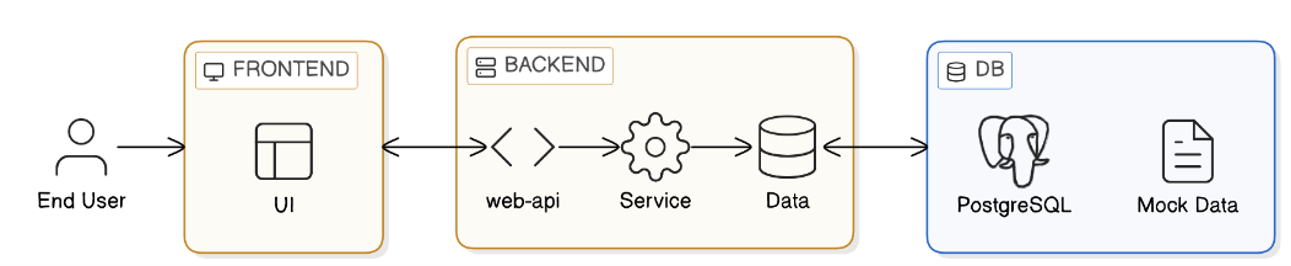
\includegraphics{./figures/system_architecture.png}}
\end{center}
\caption{System architecture diagram.}\label{fig:architecture}
\end{figure}
\FloatBarrier

As illustrated in Figure~\ref{fig:architecture}, the system is organized into three layers:

\begin{itemize}
    \item \textbf{Presentation Layer (Frontend):} built with Next.js and React, manages the complex calendar views (Agenda, Day, Week, Month, Year) and specialized interfaces for event/occurrence management, such as dynamic multi-occurrence forms.
    \item \textbf{Logic Layer (Backend):} Next.js API routes backed by a Controller-Service-Data structure (Chapter~\ref{cap:backend}): controllers parse and validate requests, services hold the core business logic and enforce role-based access (the Migration Engine, RF02, and Business Rule Engine, RF03), and the data layer abstracts all storage communication.
    \item \textbf{Data Layer (DB):} a PostgreSQL relational database provides persistent storage for events, occurrences, and system configuration, accessed through the Drizzle ORM.
\end{itemize}

All components outlined here have been implemented, including PostgreSQL, so far tested only against a local instance (Chapter~\ref{cap:deployment}). The data access layer isolates all storage behind a single point in the code, so business services never talk to the database directly, which is what makes it possible to keep an alternative JSON-based backend, currently used for the Vercel preview deployment, without any changes to the business logic, API routes, or frontend (Section~\ref{sec:data-access}).

\section{Technology Stack} \label{sec:tech-stack}

The stack was chosen to keep the whole application, frontend and backend alike, in a single TypeScript codebase, avoiding the coordination overhead of separate languages or repositories for a project of this size.

\subsection{Backend}
The backend is built on \textbf{Next.js}~\cite{nextjs} (v16, App Router), using its API routes as the HTTP entry point rather than a separate server framework. Data persistence uses \textbf{PostgreSQL}~\cite{postgresql} through \textbf{Drizzle ORM}~\cite{drizzleorm}, a TypeScript-first ORM that provides both a relational query API and raw SQL migrations (\texttt{drizzle-kit}). Request payloads are validated end-to-end with \textbf{Zod}~\cite{zod}, including schemas that are built dynamically from live database values (e.g. valid event categories). Password hashing uses Node.js's built-in \texttt{crypto} module~\cite{nodejscrypto} (scrypt), and session cookies follow the \texttt{Secure}/\texttt{HttpOnly} guidance from the OWASP Session Management Cheat Sheet~\cite{owasp}. National holiday and business-day calculations use the \texttt{date-fns} and \texttt{date-holidays} libraries. The automated test suite (Section~\ref{sec:backend-tests}) is built on \textbf{Vitest}~\cite{vitest}.

\subsection{Frontend}
The frontend is built with \textbf{React 19}~\cite{react} inside the same Next.js application (no separate frontend project), styled with \textbf{Tailwind CSS v4}~\cite{tailwindcss} and the \textbf{shadcn/ui}~\cite{shadcnui} component library (built on Radix UI primitives~\cite{radixui}). Forms use \textbf{react-hook-form}~\cite{reacthookform} together with \textbf{Zod resolvers} for validation, \textbf{sonner} provides toast notifications for asynchronous feedback, \textbf{framer-motion}~\cite{framermotion} drives the calendar's animations, the native HTML5 drag-and-drop API handles occurrence rescheduling, and \textbf{re-resizable} handles occurrence resizing. The project uses \textbf{pnpm}~\cite{pnpm} as its package manager and \textbf{TypeScript}~\cite{typescript} throughout both the frontend and backend.

\section{Data Model and Entity-Relationship Diagram} \label{sec:data-model}

To support automated year-to-year migration, rule validation, and the notification system (Section~\ref{sec:backend-notifications}), a relational database schema was designed and implemented with Drizzle ORM, visually outlined in the simplified Entity-Relationship Diagram in Figure~\ref{fig:er-diagram}, generated directly from the Drizzle schema definitions (\texttt{db/schema/auth.schema.ts}, \texttt{db/schema/calendar.schema.ts}, \texttt{db/schema/notification.schema.ts}, \texttt{db/schema/relations.ts}). This diagram shows every table and its relationships but omits column-level attributes for readability; the full version, with every column and its type, is given in Appendix~\ref{app:er-diagram}.

\begin{figure}[htbp]
\begin{center}
\resizebox{\textwidth}{!}{%
\begin{tikzpicture}[
    entity/.style={draw, rectangle, rounded corners=1pt, align=center, font=\small\bfseries, text width=2.8cm, inner sep=2mm, fill=white},
    relationship/.style={draw, diamond, aspect=3.4, font=\small, inner sep=1mm, align=center, fill=white},
    cascade/.style={thick},
    restrict/.style={thick, dashed},
    card/.style={fill=white, inner sep=1.5pt, font=\small},
]

% --- entities ---
\node[entity] (events) at (0,0) {Event};
\node[entity] (academicyears) at (-6,4.5) {Academic Year};
\node[entity] (users) at (6,4.5) {User};
\node[entity] (vacationperiods) at (-6,7.8) {Vacation Period};
\node[entity] (sessions) at (6,7.8) {Session};
\node[entity] (categories) at (-10,-4.5) {Category};
\node[entity] (classifications) at (-4,-4.5) {Classification};
\node[entity] (statuses) at (4,-4.5) {Status};
\node[entity] (responsibles) at (10,-4.5) {Responsible};
\node[entity] (occurrences) at (-2.0,-10) {Occurrence};
\node[entity] (rules) at (2,-10) {Event Rule};
\node[entity] (notifications) at (-2.0,-14) {Notification};

\node[relationship] (rel-ay-events) at ($(academicyears)!0.5!(events)$) {has};
\node[relationship] (rel-ay-vac) at ($(academicyears)!0.5!(vacationperiods)$) {has};
\node[relationship] (rel-users-events) at ($(users)!0.5!(events)$) {creates};
\node[relationship] (rel-users-sessions) at ($(users)!0.5!(sessions)$) {authenticates};
\node[relationship] (rel-events-cat) at ($(events)!0.7!(categories)$) {categorized\_as};
\node[relationship] (rel-events-class) at ($(events)!0.7!(classifications)$) {classified\_as};
\node[relationship] (rel-events-status) at ($(events)!0.7!(statuses)$) {has\_status};
\node[relationship] (rel-events-resp) at ($(events)!0.7!(responsibles)$) {assigned\_to};
\node[relationship] (rel-events-occ) at ($(events)!0.68!(occurrences)$) {has};
\node[relationship] (rel-events-rules) at ($(events)!0.68!(rules)$) {has};
\node[relationship] (rel-occ-notif) at ($(occurrences)!0.5!(notifications)$) {has};

% --- edges: entity -- diamond -- entity, with cardinalities near each entity end ---
\draw[cascade] (academicyears) -- (rel-ay-events) node[card, pos=0.2] {1};
\draw[cascade] (rel-ay-events) -- (events) node[card, pos=0.8] {N};

\draw[cascade] (academicyears) -- (rel-ay-vac) node[card, pos=0.2] {1};
\draw[cascade] (rel-ay-vac) -- (vacationperiods) node[card, pos=0.8] {N};

\draw[restrict] (users) -- (rel-users-events) node[card, pos=0.2] {1};
\draw[restrict] (rel-users-events) -- (events) node[card, pos=0.8] {N};

\draw[cascade] (users) -- (rel-users-sessions) node[card, pos=0.2] {1};
\draw[cascade] (rel-users-sessions) -- (sessions) node[card, pos=0.8] {N};

\draw[restrict] (events) -- (rel-events-cat) node[card, pos=0.2] {N};
\draw[restrict] (rel-events-cat) -- (categories) node[card, pos=0.8] {1};

\draw[restrict] (events) -- (rel-events-class) node[card, pos=0.2] {N};
\draw[restrict] (rel-events-class) -- (classifications) node[card, pos=0.8] {1};

\draw[restrict] (events) -- (rel-events-status) node[card, pos=0.2] {N};
\draw[restrict] (rel-events-status) -- (statuses) node[card, pos=0.8] {1};

\draw[restrict] (events) -- (rel-events-resp) node[card, pos=0.2] {N};
\draw[restrict] (rel-events-resp) -- (responsibles) node[card, pos=0.8] {1};

\draw[cascade] (events) -- (rel-events-occ) node[card, pos=0.2] {1};
\draw[cascade] (rel-events-occ) -- (occurrences) node[card, pos=0.8] {N};

\draw[cascade] (events) -- (rel-events-rules) node[card, pos=0.2] {1};
\draw[cascade] (rel-events-rules) -- (rules) node[card, pos=0.8] {N};

\draw[cascade] (occurrences) -- (rel-occ-notif) node[card, pos=0.2] {1};
\draw[cascade] (rel-occ-notif) -- (notifications) node[card, pos=0.8] {1};

% --- legend ---
\node[draw, align=left, font=\small, anchor=south west, fill=white] at (-9.3,9.4) {
    \tikz{\draw[cascade] (0,0) -- (0.5,0);} ON DELETE CASCADE \\
    \tikz{\draw[restrict] (0,0) -- (0.5,0);} ON DELETE NO ACTION (restrict)
};
\end{tikzpicture}%
}
\end{center}
\caption{Simplified Entity-Relationship Diagram, derived from the Drizzle schema.}\label{fig:er-diagram}
\end{figure}
\FloatBarrier

Each diamond names the relationship between the two entities it connects, with cardinalities (1/N) marked at each end. Solid lines are foreign keys with \texttt{ON DELETE CASCADE}; dashed lines are \texttt{ON DELETE NO ACTION} (the referenced row cannot be deleted while still in use). For clarity, this diagram omits the \texttt{notification\_reads} table, which tracks, per user, which notifications that user has already read; it is described in Section~\ref{sec:notification-entities} and included, with its attributes, in the appendix version of this diagram.

\subsection{Core Scheduling Entities} \label{sec:core-entities}

The system's core logic centers on the relationship between events and occurrences, plus the \texttt{academic\_years} table that anchors both to a specific year:

\begin{itemize}
    \item \textbf{Academic Year:} keyed by its start year, stores a label and the concrete \texttt{start\_date}/\texttt{end\_date} that bound the academic year.
    \item \textbf{Event:} stores high-level metadata such as the objective, category, classification, status, responsible party, and the academic year and user that own it.
    \item \textbf{Occurrence:} a concrete instance of an event, with its own \texttt{start\_date} and \texttt{end\_date}, and optional \texttt{min\_days}/\texttt{min\_days\_to\_next} constraints. Each event can have multiple occurrences, and every occurrence is deleted automatically (\texttt{ON DELETE CASCADE}) when its parent event is deleted.
\end{itemize}

\subsection{Classification and Management} \label{sec:classification-entities}

To facilitate filtering and institutional reporting, the system uses four normalization/lookup tables referenced by events: \textbf{Category} (which also stores a \texttt{color}, used to render the category badges and filter dots in the calendar UI, Section~\ref{sec:frontend-calendar-ui}), \textbf{Classification}, \textbf{Status}, and \textbf{Responsible}. Each event references one value from each of these tables, allowing events to be categorized (e.g. ``TFM'', ``Candidaturas''), tracked through a planning workflow status (e.g. ``Por Fazer'', ``Em Curso'', ``Feito''), and attributed to an owning department (e.g. ``Serviços Académicos'', ``Conselho Pedagógico''). Unlike the scheduling entities above, these reference tables are not cascade-deleted: a category, classification, status, or responsible value that is still referenced by an event cannot be removed, which prevents institutional data from silently losing its classification.

\subsection{Automation and Business Rules} \label{sec:automation-entities}

Each event can have zero or more \textbf{Event Rules} attached (\texttt{event\_rules} table), storing a rule \texttt{type} and a JSON \texttt{config} object. These rows are what the Business Rule Engine evaluates for that event (Section~\ref{sec:rule-engine}); the \textbf{Vacation Period} table, scoped to an academic year, stores the school vacation periods that both the rule engine and the migration engine consult.

\subsection{Notifications} \label{sec:notification-entities}

The \textbf{Notification} table (\texttt{notifications}) stores one row per occurrence a notification has been generated for, uniquely keyed by \texttt{occurrence\_id} so at most one exists per occurrence at a time, together with the occurrence's start date and lead time as they were at generation, \texttt{occurrence\_start\_date\_at\_gen} and \texttt{lead\_days\_at\_gen}, which is how the service (Section~\ref{sec:backend-notifications}) detects that a notification has gone stale and needs regenerating. Rather than targeting a single user, a notification is shared institution-wide; per-user read state is tracked separately in \textbf{Notification Read} (\texttt{notification\_reads}), a table with a composite primary key of \texttt{notification\_id} and \texttt{user\_id} plus a \texttt{read\_at} timestamp, so the same notification can be read by one user and still show as unread to another. Both tables cascade-delete: a Notification is removed when its Occurrence is deleted, and a Notification Read row is removed when either its Notification or its User is deleted.

\subsection{Security and Auditing} \label{sec:security-entities}

The \textbf{User} and \textbf{Session} entities manage multi-role access control. The User table stores a \texttt{scrypt}-hashed password and a role (\texttt{viewer}, \texttt{editor}, or \texttt{admin}); the Session table tracks active session tokens and their expiration, and is deleted automatically when its owning user is deleted. Every Event additionally stores the \texttt{user\_id} of its creator, providing a basic audit trail of who owns each entry in the calendar.

\section{Data Access Strategy} \label{sec:data-access}

The data access layer isolates all storage behind a repository interface per feature (\texttt{IAuthRepository}, \texttt{ICalendarRepository}, \texttt{INotificationRepository}), so that business services only ever call the interface, never a concrete database client. Two concrete implementations exist for each interface: a PostgreSQL implementation built on Drizzle ORM (\texttt{AuthRepositoryPostgres}, \texttt{CalendarRepositoryPostgres}, \texttt{NotificationRepositoryPostgres}), intended for the institutional VM deployment (Chapter~\ref{cap:deployment}), and a JSON-backed implementation on top of Upstash Redis~\cite{upstashredis} (\texttt{AuthRepositoryRedis}, \texttt{CalendarRepositoryRedis}, \texttt{NotificationRepositoryRedis}), used for the Vercel~\cite{vercel} preview deployment and local development, since it requires no remote database server to be provisioned.

Which implementation is used is decided by a small factory, selected through the \texttt{DATA\_LAYER} environment variable: any value other than the literal \texttt{"redis"} (including the variable being unset) resolves to PostgreSQL. Because every business service depends only on the repository interface, switching between the two backends requires no change to controllers, services, API routes, or the frontend; only the environment variable changes. This design was validated in practice during development, when the project moved from the JSON-backed mock data used while building the business logic to a locally-tested PostgreSQL database without touching the migration engine, the rule engine, or any UI code.


% Capitulo 4
%
% Chapter 4 - Backend
%
\chapter{Backend} \label{cap:backend}

This chapter details the backend implementation of EduCal, covering its layered organization, authentication, authorization, error handling, and testing approach.

\section{Organization} \label{sec:backend-organization}

The backend is organized per feature (\texttt{auth}, \texttt{calendar}) under \texttt{server/}, each following the same three-layer structure of Controller, Service, and Data, plus a \texttt{server/shared/} module for cross-cutting concerns (the API response envelope, domain error type, and the data-layer factory). This mirrors the Controller-Service-Repository pattern used since the initial implementation: controllers such as \texttt{authController} and \texttt{calendarController} act as orchestrators that parse and validate the incoming HTTP request and hand off to the corresponding service, keeping the route handlers in \texttt{app/api/**/route.ts} as thin wrappers, as shown in Listing~\ref{lst:api-route}.

\begin{lstlisting}[caption={[Calendar events API route.]{Calendar events API route (\texttt{app/api/events/route.ts}): each HTTP verb is wired directly to a controller method, behind the authentication middleware.}}, label={lst:api-route}]
export const GET = withApiAuth(async () => {
  return calendarController.listEvents();
});

export const POST = withApiAuth(async (request) => {
  return calendarController.createEvent(request);
});
\end{lstlisting}

Neither handler parses the request itself, checks the role, or catches errors: \texttt{withApiAuth} (Section~\ref{sec:backend-authentication}) resolves the session cookie into a user before either handler runs, and every failure, whether it comes from validation, authorization, or the database, is funnelled through the controller's own \texttt{fail()} call (Section~\ref{sec:backend-error-handling}). This keeps every route file in \texttt{app/api/} at a near-identical, one-line shape, regardless of which feature or HTTP verb it implements.

\section{Authentication} \label{sec:backend-authentication}

Passwords are never stored in plain text: they are hashed with Node.js's built-in \texttt{crypto} module~\cite{nodejscrypto} using \texttt{scrypt}, a per-password random 16-byte salt, and a 64-byte derived key, stored as \texttt{scrypt\$salt\$hash}. Password verification uses a constant-time comparison (\texttt{crypto.timingSafeEqual}) to reduce the risk of timing attacks. Listing~\ref{lst:crypto} shows the implementation of both functions.

\begin{lstlisting}[caption={[Password hashing and verification.]{Password hashing and verification (\texttt{server/auth/crypto.ts}).}}, label={lst:crypto}]
export const hashPassword = (password: string): string => {
  const salt = crypto.randomBytes(16).toString("hex");
  const hash = crypto.scryptSync(password, salt, 64).toString("hex");
  return `scrypt$${salt}$${hash}`;
};

export const verifyPassword = (password: string, encodedHash: string): boolean => {
  const [algorithm, salt, storedHash] = encodedHash.split("$");
  if (algorithm !== "scrypt" || !salt || !storedHash) {
    return false;
  }

  const computedHash = crypto.scryptSync(password, salt, 64).toString("hex");
  if (computedHash.length !== storedHash.length) return false;
  return crypto.timingSafeEqual(
    Buffer.from(storedHash, "hex"),
    Buffer.from(computedHash, "hex"),
  );
};
\end{lstlisting}

\texttt{hashPassword} generates a fresh random salt for every password and derives a 64-byte key with \texttt{scryptSync}, encoding the algorithm tag, salt, and derived key into the single \texttt{\$}-delimited string that is stored in the \texttt{users.password\_hash} column. \texttt{verifyPassword} parses that string back into its three parts, rejecting anything not tagged \texttt{scrypt} or missing a segment, then re-derives the hash from the candidate password using the stored salt and compares it against the stored hash with \texttt{crypto.timingSafeEqual}. Comparing the two hashes' lengths before calling \texttt{timingSafeEqual} avoids that function throwing on mismatched buffer sizes, while still not leaking any timing information for hashes of equal length.

On login, the service generates a random 48-byte, base64url-encoded session token and persists it, together with its expiration, in the \texttt{sessions} table. Two expiration policies are supported: a short-lived session (1 day) by default, or a 30-day session when the user selects ``Remember Me'' (\texttt{staySignedIn}). The session token is sent to the browser as a cookie that is \texttt{HttpOnly} (not accessible to client-side scripts, mitigating XSS-based token theft), \texttt{Secure} in production, and \texttt{SameSite=Lax}~\cite{owasp}; the cookie itself only carries a \texttt{maxAge} when ``Remember Me'' is selected, otherwise it is a session-only cookie. On every authenticated request, the session is also validated server-side against its stored expiration, and expired sessions are deleted rather than just ignored.

\section{Error Handling} \label{sec:backend-error-handling}

API responses follow a consistent envelope: successful responses return \texttt{\{ data: ... \}}, and failures return \texttt{\{ error: \{ code, message, details \} \}}. Domain-level failures are raised as a typed \texttt{DomainError} (with an error code such as \texttt{UNAUTHORIZED}, \texttt{FORBIDDEN}, \texttt{NOT\_FOUND}, or \texttt{CONFLICT}, and an HTTP status), and Zod validation failures are caught and converted into a \texttt{VALIDATION\_ERROR} response with a structured, field-level breakdown of what failed. Every controller method funnels its errors through this single \texttt{fail()} helper, which guarantees the frontend always receives a predictable error shape to parse and display, regardless of which layer raised the error.

\section{Role-Based Access Control} \label{sec:backend-rbac}

Three roles are supported, \texttt{viewer}, \texttt{editor}, and \texttt{admin}, ordered in a strict hierarchy. Calendar-editing operations (creating, updating, or deleting events, occurrences, and vacation periods, and running the migration engine) require at least the \texttt{editor} role; user management requires the \texttt{admin} role. Authentication itself is enforced by HTTP-level middleware (\texttt{withApiAuth}/\texttt{withApiAuthContext}) that resolves the session cookie into a user and rejects unauthenticated requests before they reach a controller; role checks are then applied one layer down, inside the services.

Rather than scattering an \texttt{if (role !== "editor") throw ...} check across each service method, role enforcement is centralized in a single generic wrapper, \texttt{withRolePolicy} (Listing~\ref{lst:with-role-policy}), applied once at the point where each service is instantiated. It takes the concrete service instance, a policy map from method name to a minimum role (or the literal \texttt{"any"} for methods with no restriction), and a \texttt{getRole} function that extracts the caller's role from that method's own arguments, since every authenticated service method already receives the caller's session as part of its first argument (Section~\ref{sec:backend-controller}). It returns a new object in which every listed method is re-wrapped to assert the minimum role before delegating to the original implementation.

\begin{lstlisting}[caption={[The withRolePolicy authorization wrapper.]{The \texttt{withRolePolicy} authorization wrapper (\texttt{server/shared/authorize.ts}).}}, label={lst:with-role-policy}]
export function withRolePolicy<
  TInstance extends object,
  TPolicy extends Partial<Record<keyof TInstance, TRolePolicy>>,
>(
  instance: TInstance,
  policy: TPolicy,
  getRole: (args: unknown[]) => TUserRole,
): { [K in keyof TPolicy]: TInstance[K & keyof TInstance] } {
  const wrapped: Record<string, unknown> = {};

  for (const key of Object.keys(policy)) {
    const minimum = policy[key as keyof TPolicy] as TRolePolicy;
    const original = instance[key as keyof TInstance] as unknown as
      (...args: unknown[]) => unknown;

    wrapped[key] = (...args: unknown[]) => {
      if (minimum !== "any") {
        assertRole(getRole(args), minimum);
      }
      return original.apply(instance, args);
    };
  }

  return wrapped as { [K in keyof TPolicy]: TInstance[K & keyof TInstance] };
}
\end{lstlisting}

The design is deny-by-default, and enforces this at the type level rather than only at runtime: a method the policy map omits is not merely left unchecked, it is absent from the returned object's TypeScript type entirely. Adding a new method to a service without adding a matching policy entry therefore fails to compile at every call site, instead of silently exposing an unauthorized method to the controllers that consume it. \texttt{calendarService} and \texttt{authService} are both exported as the result of this wrapper, each with its own policy map, for example \texttt{listEvents: "any"} alongside \texttt{createEvent: "editor"} and \texttt{migrateAcademicYear: "editor"} for \texttt{CalendarService}, mirroring the requirement, described above, that read access stays open while calendar mutation requires at least the \texttt{editor} role.

Beyond the basic role hierarchy, the system enforces three self-management invariants to prevent an institution from locking itself out of administration:
\begin{itemize}
    \item an administrator cannot demote their own account away from \texttt{admin};
    \item an administrator cannot delete their own account;
    \item the last remaining administrator cannot be demoted or deleted; the service counts existing admins before allowing either operation and rejects it if only one would remain.
\end{itemize}

\section{Layers} \label{sec:backend-layers}

Every backend feature, is organized into the same three layers, Controller, Service, and Data, each with a single, narrow responsibility and depending only on the layer directly below it. Figure~\ref{fig:layers} illustrates this flow for a single request, and the rest of this section walks through each layer in turn, using the notification feature's own controller, service, and repository as a concrete, small enough example to show in full.

\begin{figure}[htbp]
\begin{center}
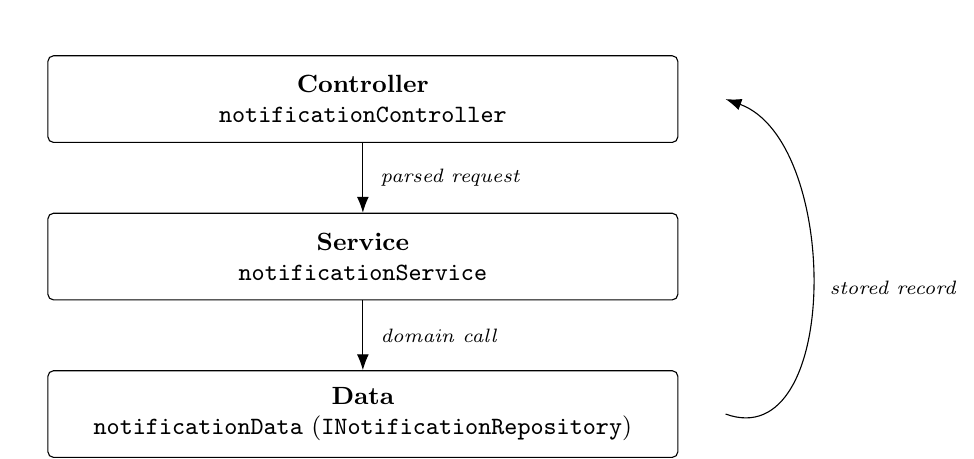
\begin{tikzpicture}[
    layer/.style={draw, rectangle, rounded corners=2pt, align=center, font=\small, minimum width=8cm, minimum height=1.1cm, fill=white},
    lbl/.style={font=\scriptsize\itshape, align=center},
]
\node[layer] (controller) at (0,4) {\textbf{Controller} \\ \texttt{notificationController}};
\node[layer] (service)    at (0,2) {\textbf{Service} \\ \texttt{notificationService}};
\node[layer] (data)       at (0,0) {\textbf{Data} \\ \texttt{notificationData} (\texttt{INotificationRepository})};

\draw[-{Latex[length=2mm]}] (controller) -- (service) node[lbl, midway, right=1mm] {parsed request};
\draw[-{Latex[length=2mm]}] (service) -- (data) node[lbl, midway, right=1mm] {domain call};
\draw[-{Latex[length=2mm]}] ($(data.east)+(0.6,0)$) to[out=-20,in=-20] node[lbl, midway, right=1mm] {stored record} ($(controller.east)+(0.6,0)$);
\end{tikzpicture}
\end{center}
\caption{The Controller-Service-Data layering, instantiated for the notification feature.}\label{fig:layers}
\end{figure}
\FloatBarrier

\subsection{Controller} \label{sec:backend-controller}
Controllers (\texttt{server/auth/controllers/}, \texttt{server/calendar/controllers/}, \texttt{server/notifications/controllers/}) are the entry point for each API route. They parse and validate route parameters and the request body, invoke the corresponding service method, and translate the result, or any error thrown, into an HTTP response using the shared \texttt{ok()}/\texttt{fail()} helpers. This is also where the session cookie is set on login and cleared on logout. Listing~\ref{lst:notification-controller} shows the notification controller's \texttt{markRead} action, a minimal case of this shape.

\begin{lstlisting}[caption={[Controller layer example.]{Controller layer example (\texttt{server/notifications/controllers/notification.controller.ts}).}}, label={lst:notification-controller}]
async markRead(request: IRequestWithAuth, notificationIdValue: string) {
  try {
    const notificationId = parseNotificationId(notificationIdValue);
    await notificationService.markRead(request, notificationId);
    return ok({ read: true });
  } catch (error) {
    return fail(error);
  }
},
\end{lstlisting}

The method does no business logic of its own: it validates that a notification id was actually supplied, delegates the read entirely to \texttt{notificationService.markRead}, and converts either outcome into the standard response envelope (Section~\ref{sec:backend-error-handling}). The \texttt{try}/\texttt{catch} boilerplate is identical across every controller action in the codebase, which is precisely what keeps the layer thin: nothing here depends on how a notification is read or where it is stored.

\subsection{Service} \label{sec:backend-service}
Services (\texttt{server/auth/services/auth.service.ts}, \texttt{server/calendar/services/calendar.service.ts}, \texttt{server/notifications/services/notification.service.ts}) hold all business logic and authorization checks, and are the bridge between the controllers and the data layer. This is where the RBAC invariants described in Section~\ref{sec:backend-rbac} are enforced, and where the central pieces of calendar business logic live: the Migration Engine (Section~\ref{sec:migration-engine}), the Business Rule Engine (Section~\ref{sec:rule-engine}), and the notification lead-time computation (Section~\ref{sec:backend-notifications}). Listing~\ref{lst:notification-service} shows the core of that last one, the per-occurrence check that decides whether a notification is due.

\begin{lstlisting}[caption={[Service layer example.]{Service layer example (\texttt{server/notifications/services/notification.service.ts}).}}, label={lst:notification-service}]
for (const event of events) {
  for (const occurrence of event.occurrences) {
    const effectiveLeadDays = occurrence.notifyDaysBeforeOverride ?? event.notifyDaysBefore;
    // ... skip if a fresh record already exists for this occurrence ...

    if (
      typeof effectiveLeadDays === "number" &&
      !alreadyGenerated &&
      occurrenceStartDate > now &&
      countWorkingDaysBetween(now, occurrenceStartDate) <= effectiveLeadDays
    ) {
      toInsert.push({ id: crypto.randomUUID(), occurrenceId: occurrence.id, /* ... */ });
    }
  }
}
\end{lstlisting}

Each occurrence's own \texttt{notifyDaysBeforeOverride} takes precedence over its parent event's \texttt{notifyDaysBefore}, falling back to it when unset; if that effective lead time is defined, the occurrence has not already started, and the number of working days remaining (reusing the same \texttt{countWorkingDaysBetween} helper the rule engine uses, Section~\ref{sec:rule-engine}) has entered that window, a notification record is queued for insertion. This runs lazily, on read (Section~\ref{sec:backend-notifications}), rather than on a schedule, so it is the service, not a background job, that decides what counts as ``due''.

\subsection{Data} \label{sec:backend-data}
The data layer (\texttt{server/auth/data/}, \texttt{server/calendar/data/}, \texttt{server/notifications/data/}) exposes a repository interface (\texttt{IAuthRepository}, \texttt{ICalendarRepository}, \texttt{INotificationRepository}) per feature, abstracting all storage access. Services depend only on this interface, never on a concrete database client, which is what enables the pluggable PostgreSQL/Redis backend described in Section~\ref{sec:data-access}. Listing~\ref{lst:notification-repository} shows the notification feature's interface in full: every method a service is allowed to call, with no mention of SQL or Redis anywhere in sight.

\begin{lstlisting}[caption={[Data layer example.]{Data layer example (\texttt{server/notifications/data/notification.repository.ts}).}}, label={lst:notification-repository}]
export interface INotificationRepository {
  listAll(): Promise<NotificationRecord[]>;
  insertMany(records: NotificationRecord[]): Promise<void>;
  deleteManyByOccurrenceIds(occurrenceIds: string[]): Promise<void>;
  listReadNotificationIdsForUser(userId: string): Promise<string[]>;
  markRead(notificationId: string, userId: string): Promise<void>;
  markAllRead(notificationIds: string[], userId: string): Promise<void>;
}
\end{lstlisting}

\texttt{NotificationRepositoryPostgres} implements this interface directly against the \texttt{notifications}/\texttt{notification\_reads} tables (Section~\ref{sec:data-model}) with Drizzle queries; \texttt{NotificationRepositoryRedis} implements the same interface against a single JSON blob in Upstash Redis.

\section{Migration Engine} \label{sec:migration-engine}

The migration of the academic calendar from one year to the next is implemented as a single service operation (\texttt{CalendarService.migrateAcademicYear}), exposed to editors and administrators through dedicated ``Validate'' and ``Migrate'' actions in the calendar header (Section~\ref{sec:frontend-academic-year-tools}).

\begin{itemize}
    \item \textbf{Vacation periods first:} for the target academic year (source year $+\ 1$), the engine migrates vacation periods before events, shifting each period's dates forward by one year so that subsequent rule checks against the target year already see the correct vacation windows.
    \item \textbf{Idempotent event migration:} every source-year event is fingerprinted from a fixed subset of its fields (name, objective, category, classification, status, responsible, owner, and each occurrence's description and dates, deliberately excluding database-generated ids). If an equivalent event already exists in the target year, it is skipped; otherwise it is cloned and inserted. This makes the operation safe to run more than once without creating duplicates.
    \item \textbf{Date shifting and leap years:} each occurrence's dates are shifted forward by one calendar year. The 29th of February is handled explicitly: if shifting the year would otherwise roll the date over into March (because the target year is not a leap year), the date is instead clamped back to the 28th of February.
    \item \textbf{Validation, not automatic correction:} immediately after an event is migrated, the full business rule set (Section~\ref{sec:rule-engine}) is run against it, and any violations, such as an occurrence now falling on a weekend or holiday, are collected into a structured report returned to the caller. The engine does not shift dates to avoid these conflicts; resolving them is left as a manual, user-driven step, guided by the issue report shown in the application (Section~\ref{sec:frontend-academic-year-tools}). The same rule-checking logic also powers the standalone ``Validate'' action, which runs a read-only check without migrating anything.
\end{itemize}

Listing~\ref{lst:shift-date} shows \texttt{shiftDateByYears}, the pure function every occurrence's start and end dates are passed through during migration, which implements the leap-year clamping described above.

\begin{lstlisting}[caption={[Date shifting with leap-year clamping.]{Date shifting with leap-year clamping (\texttt{shared/calendar/academic-year.ts}).}}, label={lst:shift-date}]
export const shiftDateByYears = (dateValue: string, years: number): string => {
  const source = new Date(dateValue);
  const target = new Date(dateValue);
  target.setUTCFullYear(source.getUTCFullYear() + years);

  if (target.getUTCMonth() !== source.getUTCMonth()) {
    target.setUTCDate(0);
  }

  return target.toISOString();
};
\end{lstlisting}

Adding one year to a date is not simply incrementing its year component: calling \texttt{setUTCFullYear} on the 29th of February of a leap year silently rolls the date forward into the 1st of March whenever the target year is not itself a leap year, since the 29th of February does not exist there. The function detects this by checking whether the resulting month still matches the source month; if it does not, the date is rolled back with \texttt{setUTCDate(0)}, which JavaScript resolves to the last day of the previous month, that is, the 28th of February. Every other date is left unaffected, since shifting a day that exists in every year by whole years never changes its month.

\section{Business Rule Engine} \label{sec:rule-engine}

A modular rule engine validates event occurrences against configurable institutional constraints. Each rule is a self-contained unit implementing a shared interface (a \texttt{validate} function that receives the event, the occurrence, its configuration, and validation context such as vacation periods and other events); the engine itself has no knowledge of what a rule checks, it only calls this function and collects the result. Rules are registered in a single, central list that the engine iterates over, with no branching logic deciding which rule applies, so new institutional rules can be added by writing one new file and registering it, without touching the migration or validation logic. This same rule registry also drives the rule-configuration UI in the event form (Section~\ref{sec:frontend-event-dialogs}), which reads each rule's field metadata to render the correct input controls.

Listing~\ref{lst:weekend-rule} shows the Weekend rule, which flags an occurrence whose start date, end date, or any date spanned by a multi-day occurrence, falls on a Saturday or Sunday. Its \texttt{fields} and \texttt{translations} entries are abbreviated in the listing: each is a small, self-descriptive object, three checkbox declarations and their labels, plus one message string per violation kind, with nothing algorithmic in either.

\begin{lstlisting}[caption={[The Weekend rule definition.]{The Weekend rule definition (\texttt{server/calendar/rules/definitions/weekend.rule.ts}).}}, label={lst:weekend-rule}]
export const weekendRule: IRuleDefinition = {
  id: "weekend",
  fields: [ /* checkStart, checkEnd, checkRange checkboxes */ ],
  translations: { /* label, field labels, and one message per violation kind */ },
  validate(_event, occurrence, config) {
    return runDayRangeCheck<true>({
      occurrence,
      config: config as WeekendConfig,
      matchDay: (day) => (isWeekend(day) ? true : undefined),
      toViolation: (field, date) => ({ fieldLabelKey: field, date, messageKey: MESSAGE_KEYS[field] }),
    });
  },
};
\end{lstlisting}

Weekend, Holiday, and Vacation period all expose the same three independent toggles, checking the start date, the end date, and every date spanned by the occurrence, differing only in \emph{what} counts as a match on a given day. This shared checkStart/checkEnd/checkRange loop is factored into a single generic helper, \texttt{runDayRangeCheck} (Listing~\ref{lst:day-range-check}), which each rule parameterizes with its own day-matching and violation-building logic instead of implementing the loop itself.

\begin{lstlisting}[caption={[The shared start/end/range check helper.]{The shared start/end/range check helper (\texttt{server/calendar/rules/utils/day-range-check.ts}).}}, label={lst:day-range-check}]
export function runDayRangeCheck<TMatch>({
  occurrence, config, matchDay, matchRange, toViolation,
}: DayRangeCheckOptions<TMatch>): IRuleViolation[] {
  const violations: IRuleViolation[] = [];
  const start = parseISO(occurrence.startDate);
  const end = parseISO(occurrence.endDate);

  if (config.checkStart) {
    const match = matchDay(start);
    if (match) violations.push(toViolation("start", occurrence.startDate, match));
  }
  // ... checkEnd follows the same shape, against `end` ...

  if (config.checkRange) {
    if (matchRange) {
      const match = matchRange(start, end);
      if (match) violations.push(toViolation("range", occurrence.startDate, match));
    } else {
      for (const day of eachDayOfInterval({ start, end })) {
        const match = matchDay(day);
        if (match) {
          violations.push(toViolation("range", day.toISOString(), match));
          break;
        }
      }
    }
  }

  return violations;
}
\end{lstlisting}

\texttt{matchDay} is the single-day predicate each rule supplies (``is this day a weekend'', ``is this day a holiday'', ``is this day inside a vacation period''), returning whatever piece of matched data \texttt{toViolation} needs to build its \texttt{messageParams} (a holiday's name, a vacation period's label, or nothing at all for the Weekend rule, whose messages need no parameters). \texttt{checkRange} defaults to walking every day in the occurrence's span with \texttt{matchDay}, stopping at the first match, which is exactly what Weekend and Holiday need; the optional \texttt{matchRange} lets a rule override that with a whole-interval check instead, which the Vacation period rule uses (Listing~\ref{lst:vacation-rule}), since a vacation period is a continuous range rather than a set of independently meaningful days, so testing the whole span for overlap in one step is the more natural check.

The \texttt{id} is the stable key stored in \texttt{event\_rules.type} and used to dispatch validation; \texttt{fields} declares the rule's three independent toggles, checking the start date, the end date, and every date in between, together with their default values, which the event form (Section~\ref{sec:frontend-event-dialogs}) reads to render the matching checkboxes with no rule-specific UI code required; \texttt{translations} supplies every user-facing string the rule needs, from its display label to one message per kind of violation, keyed by locale; and \texttt{validate} is the pure function the engine calls with the event, one of its occurrences, and this rule's configuration, returning zero or more violations. Each violation carries a message key and the specific field and date that triggered it, rather than a pre-formatted string, so the frontend can translate and render it consistently with every other rule (Section~\ref{sec:frontend-academic-year-tools}).

Seven rules are currently implemented:

\begin{itemize}
    \item \textbf{Weekend:} flags occurrences whose start, end, or intermediate dates fall on a Saturday or Sunday.
    \item \textbf{Holiday:} flags occurrences that coincide with Portuguese national holidays.
    \item \textbf{Vacation period:} flags occurrences that overlap a registered school vacation period for that academic year.
    \item \textbf{Event no-overlap:} flags occurrences whose overall date span overlaps the span of other, user-selected events.
    \item \textbf{Minimum gap to event:} enforces a minimum number of working days between the end of one event and the start of a related, user-selected event.
    \item \textbf{Minimum duration:} an always-on, built-in rule enforcing a minimum calendar-day duration for an occurrence, driven by the occurrence's own \texttt{minDays} field.
    \item \textbf{Minimum gap to next occurrence:} an always-on, built-in rule enforcing a minimum working-day gap between consecutive occurrences of the same event, driven by \texttt{minDaysToNext}.
\end{itemize}

The first five rules are selectively enabled and parameterized per event through the event creation and editing interface; the last two are always active for every occurrence and are not exposed in the rule-configuration UI (they are marked \texttt{hidden} in the rule metadata). All rules are advisory: none of them block the creation, editing, or migration of an event; violations are surfaced for manual review rather than enforced automatically. This business-rule layer is distinct from the structural, blocking validation performed by Zod on every API request (e.g. ensuring an occurrence's end date is later than its start date).

Most rules derive everything they need from the event and occurrence being validated, together with \texttt{context.allEvents}, the full set of other events, for cross-event checks such as Event no-overlap or Minimum gap to event. The Vacation period rule is the exception: instead of comparing occurrences against other occurrences, it consults \texttt{context.vacations}, a list populated from the dedicated, per-academic-year Vacation Period table (Section~\ref{sec:automation-entities}), managed independently through its own dialog (Section~\ref{sec:frontend-academic-year-tools}) rather than derived from other calendar events. Listing~\ref{lst:vacation-rule} shows its core validation logic; its \texttt{fields} and \texttt{translations}, following the same three-toggle shape as Weekend and Holiday, are abbreviated here for the same reason.

\begin{lstlisting}[caption={[The Vacation period rule's validation logic.]{The Vacation period rule's validation logic (\texttt{server/calendar/rules/definitions/vacation-period.rule.ts}).}}, label={lst:vacation-rule}]
// vacationContaining(day, vacations): first vacation period containing `day`,
// via date-fns's isWithinInterval.
// vacationOverlapping(start, end, vacations): first vacation period whose
// interval overlaps [start, end], via date-fns's areIntervalsOverlapping.
// toUtcDay(d): normalizes a Date to midnight UTC of the same calendar day.

validate(_event, occurrence, config, context) {
  const { vacations } = context;
  if (!vacations || vacations.length === 0) return [];

  return runDayRangeCheck({
    occurrence,
    config: config as VacationPeriodConfig,
    matchDay: (day) => vacationContaining(toUtcDay(day), vacations),
    matchRange: (start, end) => vacationOverlapping(toUtcDay(start), toUtcDay(end), vacations),
    toViolation: (field, date, match) => ({
      fieldLabelKey: field,
      date,
      messageKey: MESSAGE_KEYS[field],
      messageParams: { vacationLabel: match.label },
    }),
  });
},
\end{lstlisting}

Passing \texttt{matchRange} here, rather than leaving it unset as the Weekend rule does, makes \texttt{checkRange} test whether the occurrence's whole span overlaps any vacation period as a single interval check, rather than \texttt{runDayRangeCheck}'s default day-by-day walk; the two are not the same computation, and only the interval form matches what ``the occurrence overlaps a vacation period'' actually means. Unlike the Weekend rule, every violation here carries a \texttt{messageParams.vacationLabel}, the specific vacation period that was matched, so the frontend can name it in the rendered message (e.g. ``The end coincides with the vacation period `Christmas break'\thinspace'') instead of only stating that a vacation conflict exists. The Holiday rule (\texttt{server/calendar/rules/definitions/holiday.rule.ts}) follows the same adapter shape as the Vacation period rule, supplying \texttt{date-holidays}' \texttt{isHoliday} lookup as its \texttt{matchDay} and a \texttt{holidayName} as its message parameter, and is omitted here since it introduces no new pattern.

Individual rule definitions are only half of the engine: something still has to decide, for every occurrence of every event in an academic year, which rules apply and collect what they return into a single report. That is the job of \texttt{CalendarService.collectEventRuleIssues} (Listing~\ref{lst:collect-issues}), a private method that is the actual entry point of the Business Rule Engine and the piece both \texttt{validateAcademicYear} and \texttt{migrateAcademicYear} (Section~\ref{sec:migration-engine}) call to produce their issue reports.

\begin{lstlisting}[caption={[The global rule-validation dispatcher.]{The global rule-validation dispatcher (\texttt{server/calendar/services/calendar.service.ts}).}}, label={lst:collect-issues}]
private collectEventRuleIssues(
  event: IEvent,
  academicYearStart: number,
  allEvents: IEvent[],
  vacations: IVacationPeriod[] = [],
): ICalendarRuleIssue[] {
  const context = { allEvents, academicYearStart, vacations };
  const issues: ICalendarRuleIssue[] = [];
  const sortedOccurrences = [...event.occurrences].sort(/* by startDate */);

  // pushIssues(occurrence, ruleType, violations) flattens each violation
  // returned by a rule into a self-contained ICalendarRuleIssue and appends
  // it to `issues`; omitted here, shown inline in the source file.

  for (const occurrence of sortedOccurrences) {
    for (const builtInRule of [minDurationRule, minDaysToNextRule]) {
      pushIssues(occurrence, builtInRule.id, builtInRule.validate(event, occurrence, {}, context));
    }

    for (const rule of (event.rules ?? [])) {
      pushIssues(occurrence, rule.type, validateEventRule(rule, event, occurrence, context));
    }
  }

  return issues;
}
\end{lstlisting}

A single \texttt{context} object, the \texttt{allEvents}/\texttt{academicYearStart}/\texttt{vacations} triple every rule's \texttt{validate} function receives as its fourth argument, is built once per event and shared by every rule invocation for that event, which is what lets rules such as Event no-overlap or Vacation period compare an occurrence against the rest of the calendar without each rule having to fetch its own data. Occurrences are sorted chronologically first so that reported issues follow a predictable order regardless of how they were entered. \texttt{pushIssues} is a small local closure that copies the event and occurrence's identifying details onto every violation it is given, which is what lets both call sites below it, the two always-on built-in rules and every rule explicitly attached to the event through \texttt{validateEventRule} (Section~\ref{sec:rule-engine}), share the same object-construction logic instead of repeating it once per rule kind. Because \texttt{validateAcademicYear} and \texttt{migrateAcademicYear} both call this exact method, a read-only ``Validate'' check and the automatic check that runs immediately after migrating an event can never disagree about what counts as a violation.

\section{Notifications} \label{sec:backend-notifications}

Beyond validating dates against institutional rules, EduCal also reminds users of occurrences that are coming up soon, through an in-app notification system rather than the email-based templates originally scoped under RF04 (Section~\ref{sec:functional-requirements}); the remaining, undelivered part of that requirement is discussed in Chapter~\ref{cap:future-work}.

Each event carries a default lead time, \texttt{notifyDaysBefore}, and any of its occurrences may override it with its own \texttt{notifyDaysBeforeOverride}, both configured directly in the event/occurrence form (Section~\ref{sec:frontend-event-dialogs}). \texttt{NotificationService} does not generate notifications on a schedule or background job; instead, \texttt{ensureGenerated} (Listing~\ref{lst:notification-service}) runs lazily, on every read (\texttt{listMine}, \texttt{markAllRead}), comparing the current date against each occurrence's effective lead time in working days. A notification, once generated, is a single row shared by every user, keyed uniquely by \texttt{occurrenceId}; read status is tracked separately, per user, in \texttt{notification\_reads} (Section~\ref{sec:data-model}), so marking a notification read for one user never affects whether another user still sees it as unread. If an occurrence's date or effective lead time changes after a notification was already generated for it, the stale record is deleted so it can be regenerated against the new value, and notifications for occurrences that no longer exist are cleaned up the same way.

\section{Tests} \label{sec:backend-tests}

An automated test suite, built with Vitest~\cite{vitest}, now covers the system's pure-logic layer: code with no database or network dependency, which is where the project's business-critical logic is concentrated. This comprises the seven business rules, the shared \texttt{runDayRangeCheck} helper they build on (Section~\ref{sec:rule-engine}), and the rule dispatcher; the working-day calculation utility that two of those rules depend on; the password hashing and verification functions and the \texttt{withRolePolicy} authorization wrapper (Section~\ref{sec:backend-authentication} and~\ref{sec:backend-rbac}); the academic-year date helpers used by the Migration Engine (Section~\ref{sec:migration-engine}); and the notification service's lead-time and staleness logic (Section~\ref{sec:backend-notifications}), exercised against an in-memory fake of its repository dependencies rather than a real database. The suite comprises 13 test files and 79 tests, all passing, reaching approximately 98\% statement coverage on the files it targets, as measured by \texttt{@vitest/coverage-v8}.

Two choices keep the suite deterministic across machines and CI runs rather than dependent on the current date or the host's timezone: the test process's timezone is pinned to UTC, and test cases use fixed calendar dates, including real Portuguese public holidays and known weekend dates, instead of computing them relative to ``today''.

The service layer, the repository/data-access layer (both the PostgreSQL and Redis implementations), API routes, and the React frontend are covered by manual testing: exercising each functional requirement's flows (event and occurrence CRUD, the migration engine, rule validation, login, and user management) directly through the application's UI and, for API endpoints, through direct HTTP requests.

The application was also tried by a small group of ISEL academic staff, the system's intended end users, who used it on their own initiative rather than following a guided script. Their feedback, gathered through punctual meetings scheduled after each item was implemented and tested, was generally positive and led to a number of user-interface adjustments.


% Capitulo 5
%
% Chapter 5 - Frontend
%
\chapter{Frontend} \label{cap:frontend}

This chapter describes the frontend implementation of EduCal: how the codebase is organized, how it communicates with the backend, and every screen and dialog that makes up the application.

\section{Structural Organization} \label{sec:frontend-organization}

EduCal is a single Next.js application (App Router) that hosts both frontend and backend, rather than two separate projects. The \texttt{app/} directory is kept as a thin routing layer (the calendar home page, the login page, the admin users page, and the API route handlers under \texttt{app/api/}), while the actual UI is organized by feature under \texttt{features/}: \texttt{features/calendar/} (the calendar itself, including views, dialogs, header controls, drag-and-drop, and settings), \texttt{features/auth/} (the login form), and \texttt{features/admin-users/} (the user management dashboard). Reusable, feature-agnostic UI primitives (buttons, dialogs, forms, selects, etc.) live under \texttt{components/ui/}, sourced and adapted from \textbf{shadcn/ui} rather than installed as a compiled dependency, and code shared between client and server (types, Zod schemas, role logic) lives under \texttt{shared/}.

\section{API Communication Architecture} \label{sec:frontend-api}

EduCal deliberately does not use HTTP API routes for reading data. Server components fetch data directly by calling backend services: \texttt{features/calendar/requests.ts}, marked \texttt{"server-only"}, is invoked once from the \texttt{Calendar} server component, and the result (events, users, enum values, vacations) is passed down as initial props into a React context provider (\texttt{CalendarProvider}), avoiding a network round-trip for the common case of simply loading the calendar.

Mutations (creating or editing an event, logging in, managing users) do go through HTTP: a shared fetch wrapper (\texttt{lib/api-client.ts}) attaches the JSON content type, unwraps the \texttt{\{ data: ... \}} envelope on success, and on failure parses the backend's error envelope (Chapter~\ref{cap:backend}) into a user-facing, translated error message. Feature-specific request modules build on this wrapper per mutation endpoint. Components call these functions inside a try/catch and surface the result as a \texttt{sonner} toast, giving immediate feedback without a full page reload.

\section{Web Application} \label{sec:frontend-web-app}

This section walks through the application as a signed-in user experiences it: how routes are protected, how a session is established, and every screen, dialog, and persistent UI element (such as the notification bell, Section~\ref{sec:frontend-notifications}) that makes up the calendar itself.

\subsection{Navigation and Access Control} \label{sec:frontend-navigation}
The application has three main routes: the calendar (\texttt{/}), the login page (\texttt{/login}), and the admin users page (\texttt{/admin/users}). Route-level access control is handled entirely on the server, in the page component itself, rather than by a client-side auth context: \texttt{app/page.tsx} resolves the current session and redirects to \texttt{/login} if none exists, before any calendar markup is ever sent to the client; \texttt{app/login/page.tsx} redirects an already-authenticated user straight to \texttt{/}; and \texttt{app/admin/users/page.tsx} redirects to \texttt{/login} if unauthenticated and to \texttt{/} if the current user is not an \texttt{admin}. On the calendar page, once the session check passes, the actual event/user/enum/vacation data is fetched inside the \texttt{Calendar} component behind a \texttt{Suspense} boundary, which shows a loading skeleton while it resolves.

\subsection{Notification Bell} \label{sec:frontend-notifications}
Once authenticated, every page shows a bell icon in the global navbar, backed by the notification system described in Section~\ref{sec:backend-notifications}. \texttt{NotificationBell} polls \texttt{GET /api/notifications} every 60 seconds and keeps an unread-count badge on the icon; opening it lists each unread notification's occurrence description and date, with a ``mark all read'' shortcut. Clicking one marks it read and navigates to \texttt{/?openEventId=\ldots\&openOccurrenceId=\ldots}; \texttt{NotificationEventOpener} watches those parameters and, once resolved against the loaded calendar context, opens that event directly in the read-only Event Details dialog (Section~\ref{sec:frontend-event-dialogs}), skipping any manual search.

\subsection{Authentication} \label{sec:frontend-auth}
Figure~\ref{fig:login} shows the login form, which has three fields: \texttt{email}, \texttt{password}, and a ``Remember Me'' checkbox (\texttt{staySignedIn}, checked by default) that controls how long the session cookie persists (Section~\ref{sec:backend-authentication}). Fields are validated client-side with the same Zod schema shape used server-side, highlighting invalid fields in red. On submit, the button switches to a disabled ``submitting…'' state; on success the app navigates back to the calendar and refreshes its server components so the newly authenticated session is picked up immediately; on failure, the server's error message is shown inline below the form, rather than as a toast.

\begin{figure}[htbp]
\begin{center}
\resizebox{95mm}{!}{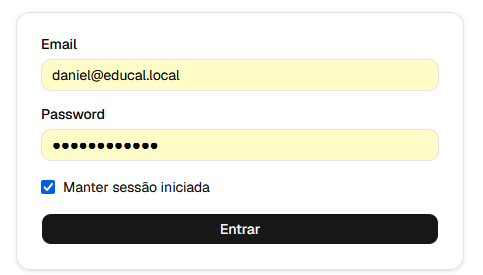
\includegraphics{./figures/app_screenshots/login_interface.png}}
\end{center}
\caption{Login interface.}\label{fig:login}
\end{figure}
\FloatBarrier

\subsection{Calendar Interface} \label{sec:frontend-calendar-ui}
The interactive calendar (Figure~\ref{fig:calendar}) is the core of the application. Its header is split into two rows: a top row with a ``Today'' shortcut and a date navigator (showing the current month/year, an event-count badge for the visible period, and previous/next controls), and an actions row containing the category filter, the Agenda/Day/Week/Month/Year view switcher, the academic-year tools (Section~\ref{sec:frontend-academic-year-tools}), a user filter, the ``Add Event'' button, and the settings menu.

The five views (\textbf{Agenda}, \textbf{Day}, \textbf{Week}, \textbf{Month}, \textbf{Year}; the latter shown in Figure~\ref{fig:calendar}, the rest in Appendix~\ref{app:calendar-views}) offer different levels of temporal density, from a scrollable list grouped by date or category (Agenda) to a full-year grid overview (Year). Within the day/week grid views, occurrences can be rescheduled directly by dragging them to a different time slot, or resized to change their duration, both implemented with the native HTML5 drag-and-drop API and animated with \texttt{framer-motion}; both actions persist immediately through the mutation flow described in Section~\ref{sec:frontend-api}. When a month-view day has more occurrences than can be shown inline, an ``+N more'' control opens a simple list dialog for that day, from which any occurrence can be opened in full detail.

The \texttt{DraggableEvent} component wraps every occurrence block shown in the day and week views, connecting the browser's native drag events to the shared drag-and-drop context (full source in Appendix~\ref{app:draggable-event}, Listing~\ref{lst:draggable-event-full}). It falls back to rendering its children unwrapped, with no drag handlers, for users without editing rights (\texttt{canEditEvents}); otherwise a native \texttt{draggable} \texttt{motion.div} dims itself while being dragged and notifies a shared drag context via \texttt{onDragStart}/\texttt{onDragEnd}. The drop target and resulting date/time update are handled by the companion \texttt{DroppableArea} component and the \texttt{updateOccurrence} mutation (Section~\ref{sec:frontend-api}).

Two controls narrow down what is shown: a category filter (multi-select dropdown, one entry per \texttt{Category}, each with its colored dot) and a user filter (single-select, showing every user's avatar and name, defaulting to ``All users''). A settings menu offers independent toggles for dark/light theme, category badge style (colored block vs. small dot), 12/24-hour time format, and how the Agenda view groups events (by date or by category), all persisted locally per browser.

\begin{figure}[htbp]
\begin{center}
\resizebox{\textwidth}{!}{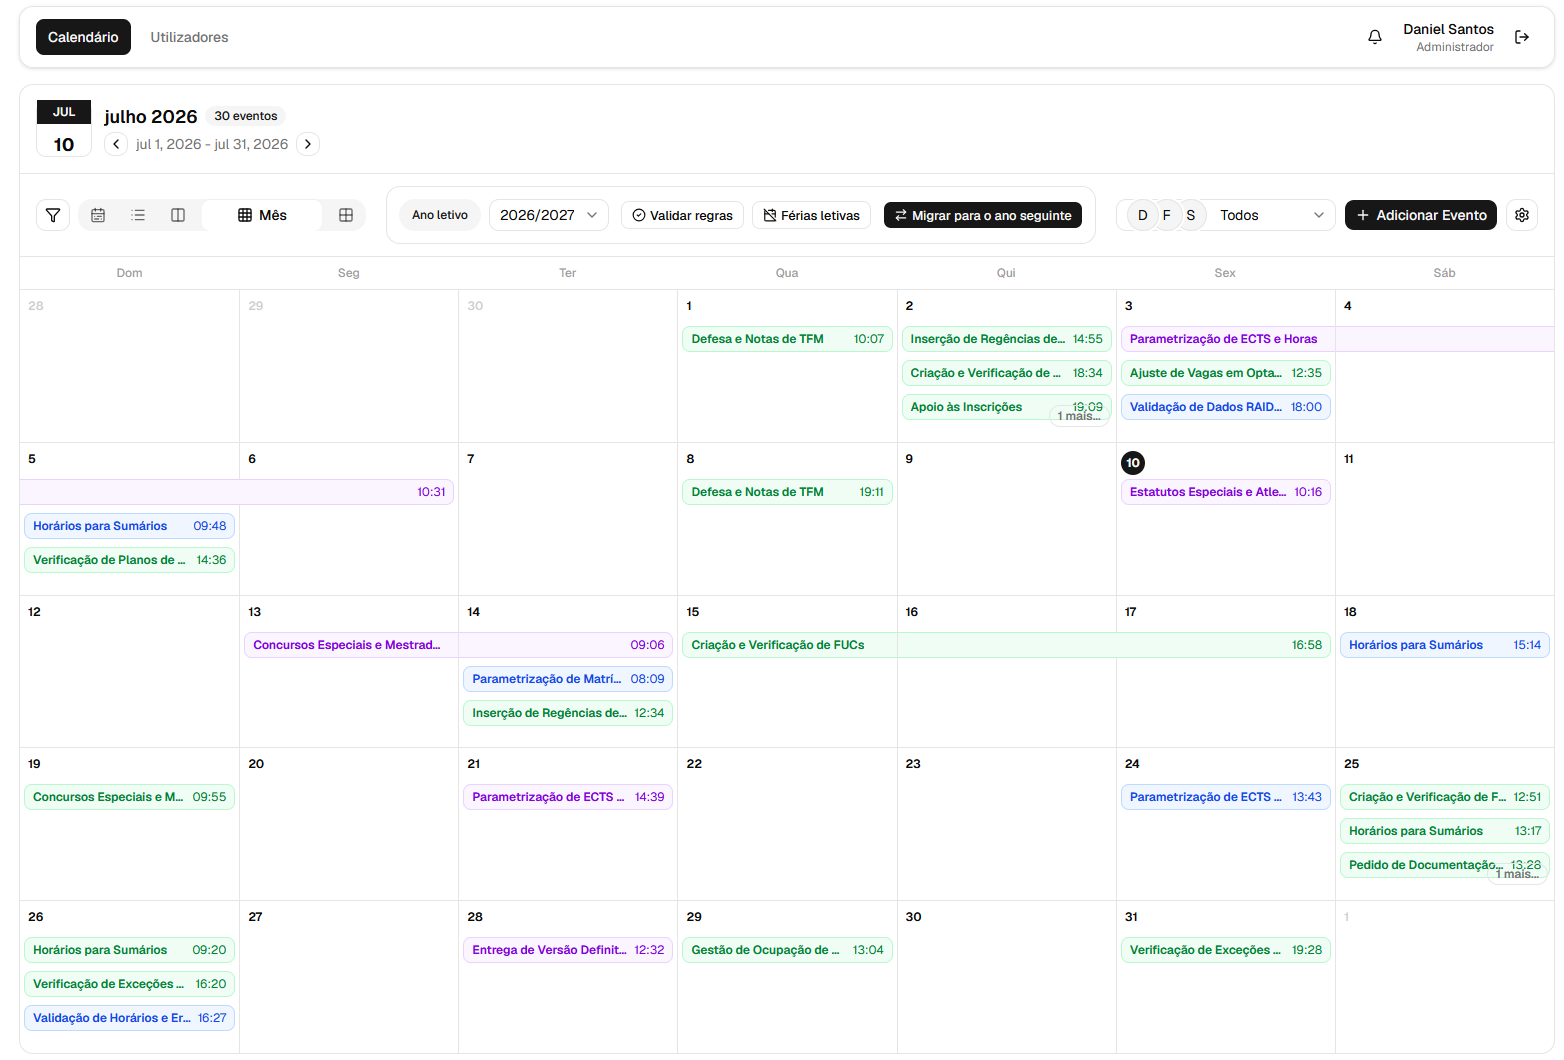
\includegraphics{./figures/app_screenshots/calendar_View.png}}
\end{center}
\caption{Main calendar interface (Month view).}\label{fig:calendar}
\end{figure}
\FloatBarrier

\subsection{Event Management Dialogs} \label{sec:frontend-event-dialogs}
The \textbf{Add/Edit Event dialog} (Figure~\ref{fig:add-edit-event}) is a single form reused for both creating and editing an event, visible only to editors and above. It has an event-level panel (\texttt{name}, \texttt{objective}, \texttt{category}/\texttt{classification}/\texttt{status}/\texttt{responsible} dropdowns, and a default notification lead time, \texttt{notifyDaysBefore}, Section~\ref{sec:backend-notifications}); an occurrence panel, a repeatable list (at least one required) each with its own \texttt{description}, \texttt{start}/\texttt{end date-time}, optional min-duration/min-gap constraints, and its own lead-time override (\texttt{notifyDaysBeforeOverride}); and a ``Rules'' panel attaching any of the five configurable business rules (Section~\ref{sec:rule-engine}), each rendering its own input controls from that rule's field metadata.

\begin{figure}[htbp]
\begin{center}
\resizebox{\textwidth}{!}{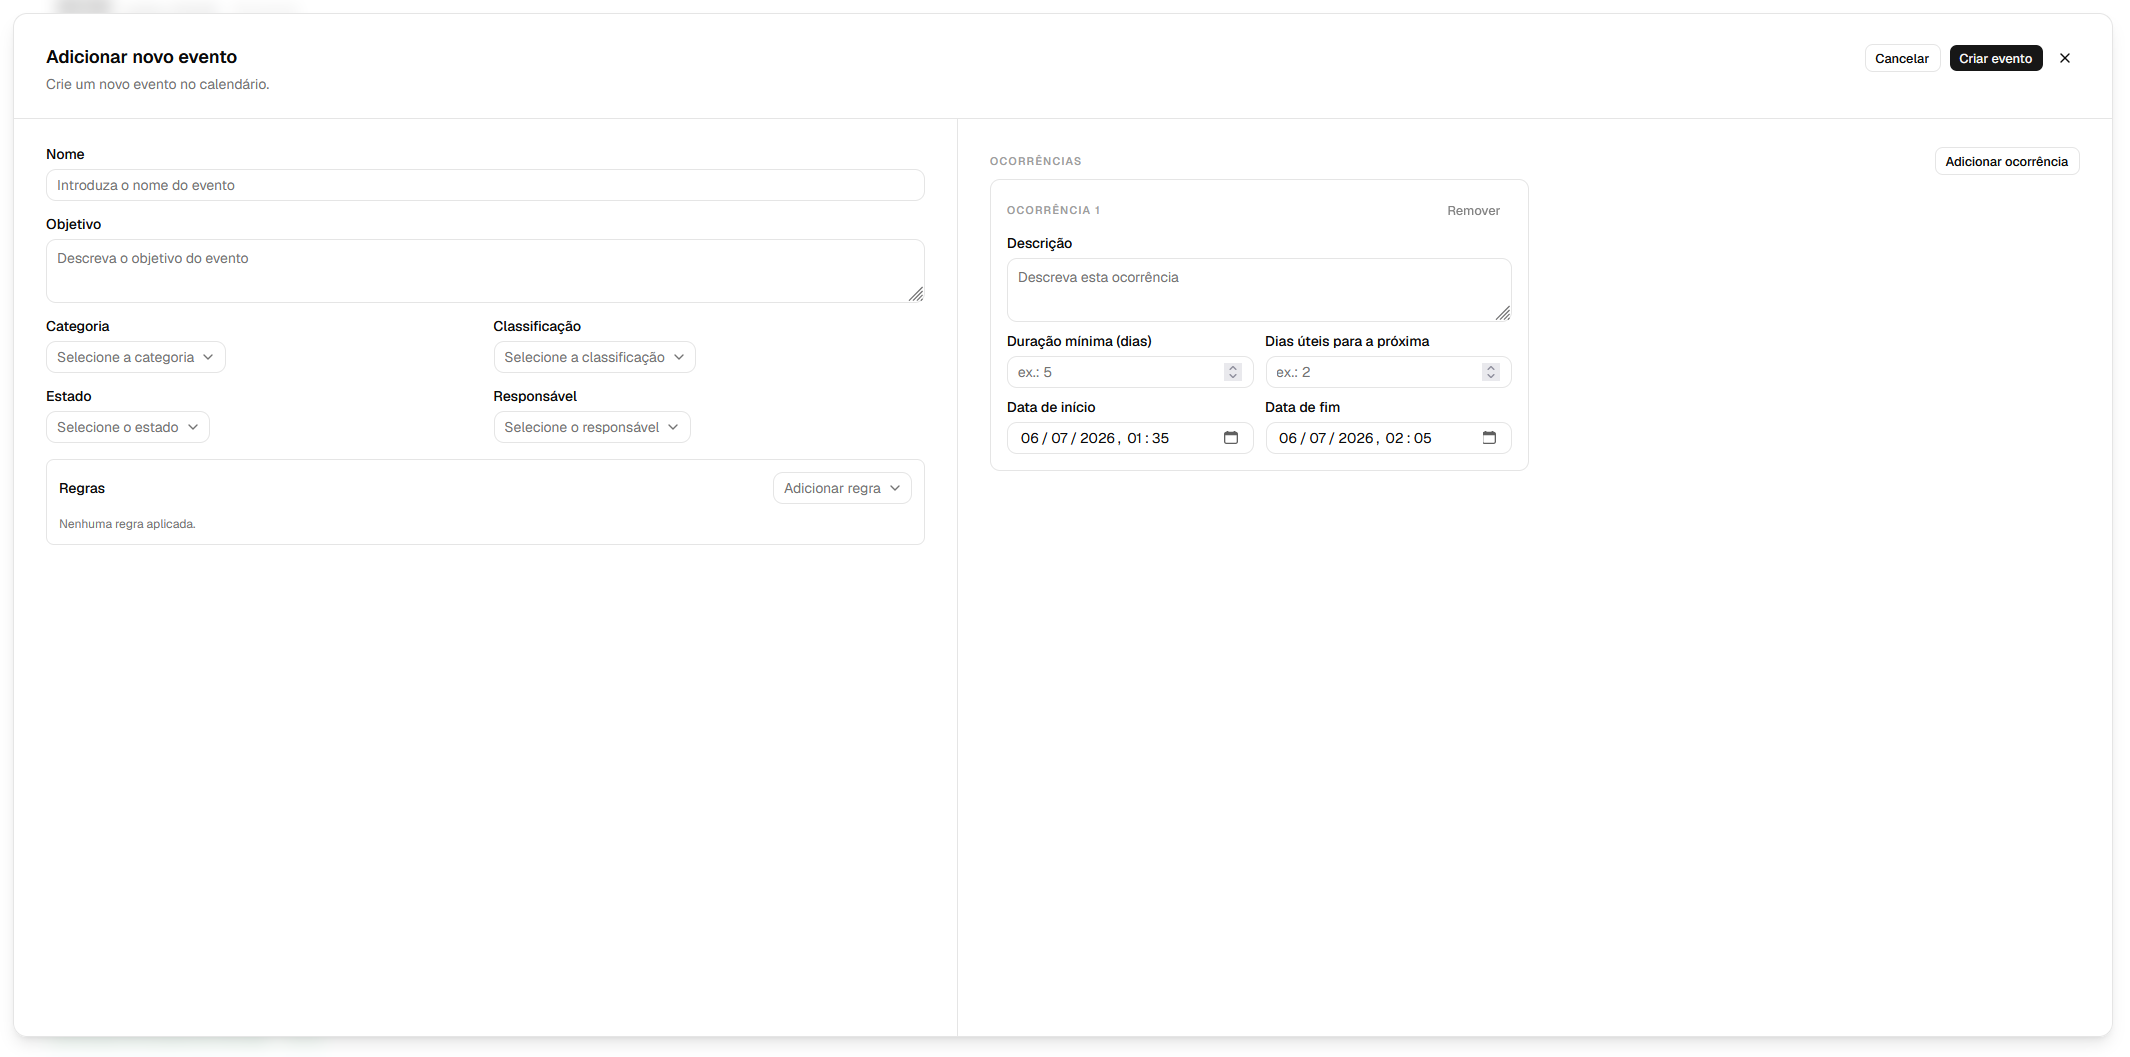
\includegraphics{./figures/app_screenshots/add_edit_event.png}}
\end{center}
\caption{Add/Edit Event dialog.}\label{fig:add-edit-event}
\end{figure}
\FloatBarrier

The \textbf{Event Details dialog} (Figure~\ref{fig:event-details}) is the read-only counterpart, opened when a user clicks an occurrence anywhere in the calendar. It shows the event's name, category/classification/status badges, its objective, who created it, the selected occurrence's dates, every occurrence in a scrollable grid, and a summary of the rules attached to the event, in the same terms an end user configured them in. Users with edit rights see shortcuts here to open the Edit dialog or delete the event directly.

\begin{figure}[htbp]
\begin{center}
\resizebox{\textwidth}{!}{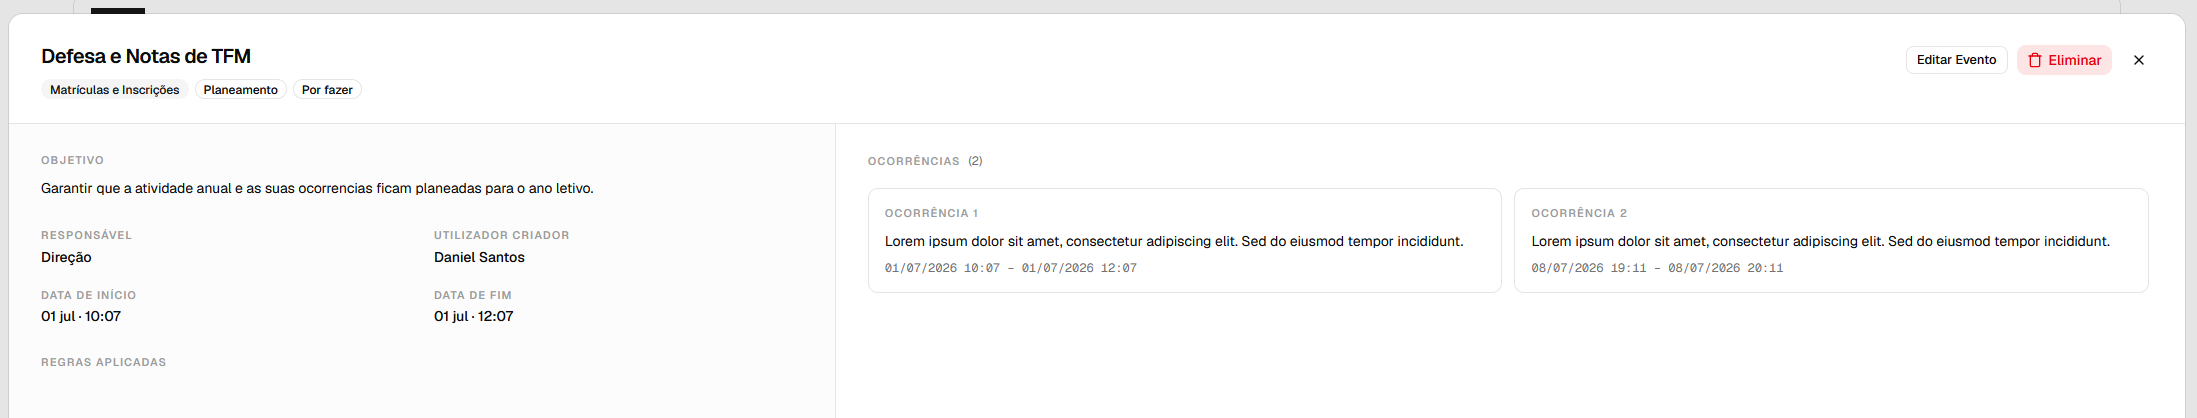
\includegraphics{./figures/app_screenshots/event_details.png}}
\end{center}
\caption{Event Details dialog.}\label{fig:event-details}
\end{figure}
\FloatBarrier

Deleting an event goes through a dedicated \textbf{confirmation dialog} (a destructive-styled button that opens an alert requiring explicit confirmation) before the event and all of its occurrences are removed, since occurrence deletion cascades from the event at the database level (Section~\ref{sec:data-model}).

\subsection{Academic Year Tools} \label{sec:frontend-academic-year-tools}
The academic-year tools, part of the calendar's actions bar, let the user pick an academic year and run the migration workflow described in Section~\ref{sec:migration-engine}: ``Validate'' checks the selected year's events against every business rule without changing anything, and ``Migrate'' (editors and administrators only) runs the full migration. Both share a results modal (Appendix~\ref{app:screenshots}, Figure~\ref{fig:migration-report-full}): a confirmation banner if no violations were found, or one card per violation otherwise, naming the rule, the affected event/occurrence, and the offending date, opening that event's Details dialog on click. A separate ``Vacations'' action opens a dedicated dialog (Figure~\ref{fig:vacations}) for managing that year's vacation periods, with full create/edit/delete support for editors.

\begin{figure}[htbp]
\begin{center}
\resizebox{90mm}{!}{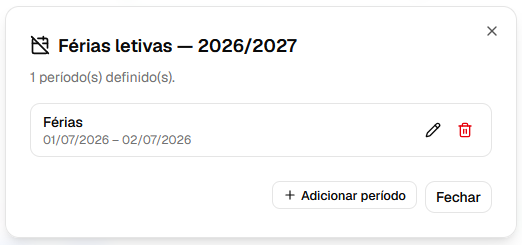
\includegraphics{./figures/app_screenshots/vacations_dialog.png}}
\end{center}
\caption{Vacation periods dialog.}\label{fig:vacations}
\end{figure}
\FloatBarrier

\subsection{User Management Dashboard} \label{sec:frontend-user-mgmt}
The administrative dashboard (Figure~\ref{fig:user-mgmt}), accessible only to administrators, lists every user in a table (name, email, role, profile picture, and actions) and supports full CRUD, with the password field left blank on edit meaning ``keep the current password''. Every mutation gives immediate toast feedback, deletions are confirmed before proceeding, and the delete action is disabled for the currently logged-in administrator's own row, reinforcing the ``cannot delete self'' invariant already enforced on the backend (Section~\ref{sec:backend-rbac}).

\begin{figure}[htbp]
\begin{center}
\resizebox{\textwidth}{!}{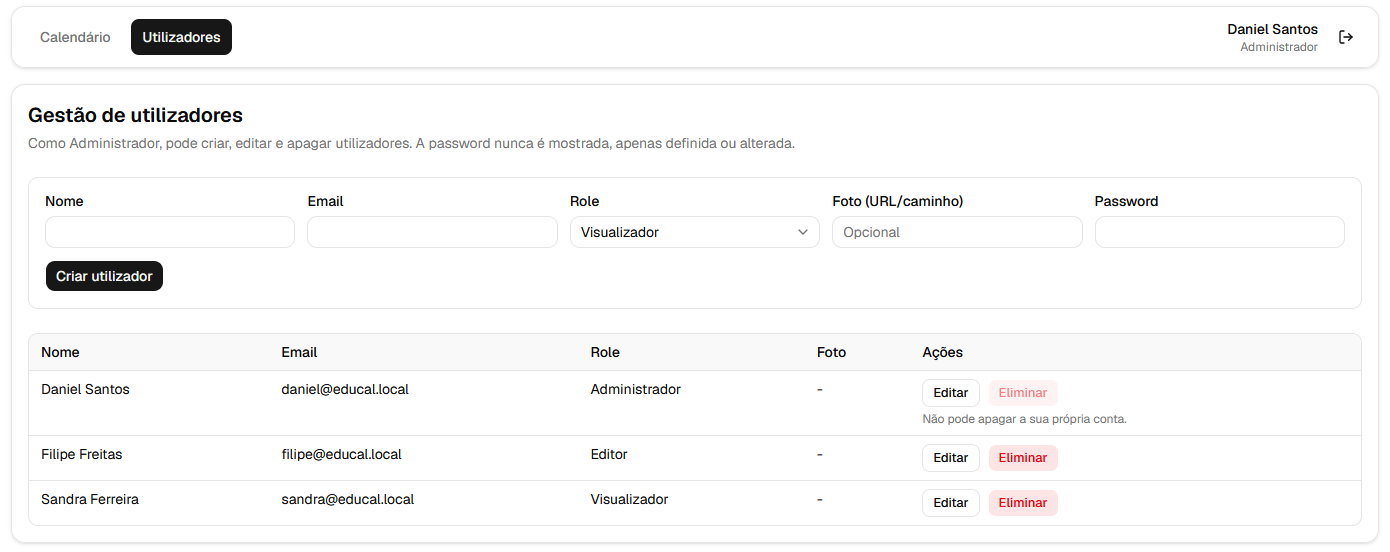
\includegraphics{./figures/app_screenshots/user_management.png}}
\end{center}
\caption{User management dashboard.}\label{fig:user-mgmt}
\end{figure}
\FloatBarrier


% Capitulo 6
%
% Chapter 6 - Deployment and Infrastructure
%
\chapter{Deployment and Infrastructure} \label{cap:deployment}

\section{Current Infrastructure} \label{sec:current-infra}

During development, EduCal was run and previewed using \textbf{Vercel}, the managed hosting platform built by the creators of Next.js. Being a zero-configuration target for Next.js applications, Vercel made it possible to get a working, publicly reachable deployment of each iteration of the application with minimal setup, which was useful for reviewing progress throughout the project without needing to provision any institutional infrastructure up front. The PostgreSQL database is accessed through a single \texttt{DATABASE\_URL} connection string, keeping the application decoupled from where the database itself is actually hosted.

Locally, the project is run with the standard Next.js toolchain, managed through \texttt{pnpm}: \texttt{pnpm dev} for the development server, and \texttt{pnpm build}/\texttt{pnpm start} to build and run a production Node.js server. There is currently no containerization (no Dockerfile) and no continuous integration/deployment pipeline configured in the repository -- builds and database migrations (\texttt{pnpm run db:migrate}) are run manually.

\section{Deployment Roadmap} \label{sec:deployment-roadmap}

Because EduCal manages institutional academic planning data, the intended production deployment is a virtual machine hosted within \textbf{ISEL's own internal network}, rather than a third-party cloud platform, so that both the application and the database remain under the institution's direct control. This VM would host the Next.js application (built and run with \texttt{pnpm build}/\texttt{pnpm start}) alongside the PostgreSQL instance.

This step has not been carried out yet: no VM has been provisioned or configured as part of this project's delivery, and there is no containerization or deployment automation in place to support it. Setting up the ISEL VM, migrating the database to it, and defining a repeatable deployment process are the concrete next steps once such infrastructure is made available by the institution.


% Capitulo 7
%
% Chapter 7 - Future Work
%
\chapter{Future Work} \label{cap:future-work}

This chapter collects the parts of the original project scope that were not delivered within the project timeline, together with the concrete next step for moving the application from its current local/Vercel setup (Chapter~\ref{cap:deployment}) into institutional use. Each of these is scoped as a follow-up to the work already completed, rather than a redesign of it: the underlying architecture (Chapter~\ref{cap:architecture}) was built to accommodate all three without further structural change.

\section{Schedule Export (RF05)} \label{sec:future-export}

RF05 (Section~\ref{sec:functional-requirements}) requires the system to generate an academic calendar in Excel format for institutional distribution; no such export exists in the current codebase. A spreadsheet suits institutional distribution better than a static rendering of the calendar UI would: recipients can sort, filter, and re-organize a schedule of events and occurrences in a way a fixed page layout does not allow. The natural shape for this is one worksheet per academic year, with one row per occurrence and a column for each piece of metadata already modeled on the event and occurrence (name, category, classification, status, responsible, description, and dates), built with a library such as \texttt{exceljs}, which produces a native \texttt{.xlsx} workbook directly from TypeScript objects. This would follow the same Controller-Service-Data shape as the rest of the backend (Section~\ref{sec:backend-layers}): a new service method assembling the relevant events and occurrences for a given academic year and category selection, and a controller action streaming the resulting workbook back as the HTTP response.

\section{Email Notification Templates (remaining RF04 scope)} \label{sec:future-notification-templates}

RF04 originally called for configurable email or other text templates associated with events, for sending proactive notifications. The in-app half of this requirement was delivered (Section~\ref{sec:backend-notifications}): EduCal now surfaces upcoming occurrences to signed-in users through the notification bell (Section~\ref{sec:frontend-notifications}), based on a configurable per-event or per-occurrence lead time. What remains is the template half of the original requirement: a free-text field, attached to an event, that an editor could fill in with the wording of a reminder (for example, the exact phrasing to send to a department ahead of an enrolment deadline), and a way to surface that text so a staff member could copy it and send it manually through the institution's own email system; it remains future work purely because it was not reached within the project timeline, not because of any technical obstacle identified during development.

\section{Deployment to the ISEL Virtual Machine} \label{sec:future-deployment}

The application currently runs from a local development environment and a Vercel preview deployment backed by the Redis-based data layer (Section~\ref{sec:current-infra}); PostgreSQL, the storage backend the institutional deployment is meant to use, has only been exercised locally. Chapter~\ref{cap:deployment} already lays out the intended production setup, a single virtual machine on ISEL's internal network hosting both the Next.js application and PostgreSQL, and the concrete steps to provision it (Section~\ref{sec:deployment-roadmap}). None of those steps have been carried out yet, because of timeline constraints but, the immediate next steps are running the Drizzle migrations against the new database, seeding its reference lookup tables and initial administrator account, and putting the application behind a process manager and reverse proxy so it survives restarts and serves traffic over HTTPS. Establishing a recurring PostgreSQL backup schedule at that point, rather than after the calendar is already in active use, would close the last gap between the current delivery and a production-ready deployment.


% Capitulo 8
%
% Chapter 8 - Conclusion
%
\chapter{Conclusion} \label{cap:conclusion}

At the conclusion of the project timeline, EduCal has moved from a conceptual set of requirements to a functional web application that replaces the spreadsheet-based process previously used for institutional academic planning at ISEL (Chapter~\ref{cap:background}). Of the six functional requirements defined in Section~\ref{sec:functional-requirements}, four were fully implemented and are in use: hierarchical event and occurrence management (RF01, Sections~\ref{sec:core-entities} and~\ref{sec:frontend-event-dialogs}), the idempotent, rule-aware academic-year Migration Engine (RF02, Section~\ref{sec:migration-engine}), the configurable Business Rule Engine (RF03, Section~\ref{sec:rule-engine}), and role-based multi-user access control (RF06, Sections~\ref{sec:backend-authentication}, \ref{sec:backend-rbac}, and~\ref{sec:frontend-user-mgmt}). Two requirements from the original scope were not delivered: notification templates (RF04) and PDF schedule export (RF05); no corresponding functionality exists in the current codebase, and both are excluded from this delivery.

The decision to structure the backend as a decoupled Controller-Service-Data pipeline, with all storage access hidden behind a repository interface (Section~\ref{sec:data-access}), proved effective throughout the project. It allowed the migration engine and the rule engine to be built and iterated on independently of the underlying data store, and it made the transition from the JSON-backed mock data used while developing the business logic to the production PostgreSQL database a matter of changing a single environment variable, with no changes required to the controllers, services, API routes, or frontend. The same separation is what makes it possible to keep the lightweight Redis-backed implementation alongside PostgreSQL for development and demos, without either implementation leaking into the rest of the system.

Overall, EduCal delivers a reliable, working solution for the core problem stated in Chapter~\ref{cap:background} -- eliminating the manual, error-prone, spreadsheet-based rebuilding of the academic calendar every year -- through automated migration and configurable rule enforcement, backed by a secure, role-based multi-user system. Completing notification templates and schedule export, and moving from the current local/Vercel setup to the planned ISEL VM deployment (Chapter~\ref{cap:deployment}), remain as the identified gaps between this delivery and the full original scope.


% Referências
\bibliographystyle{unsrt}
\bibliography{referencias}
\addcontentsline{toc}{chapter}{References}

% Apêndices
\appendix
%
% Appendix A - Detailed Entity-Relationship Diagram
%
\chapter{Detailed Entity-Relationship Diagram} \label{app:er-diagram}

This appendix presents the full version of the Entity-Relationship Diagram introduced in Section~\ref{sec:data-model} (Figure~\ref{fig:er-diagram}), including every table's columns, types, and key annotations, generated from the same Drizzle schema definitions. Relationship lines carry the same cardinality convention used in the main body: \texttt{1}/\texttt{N} at each end, solid for \texttt{ON DELETE CASCADE}, dashed for \texttt{ON DELETE NO ACTION}.

\begin{landscape}
\begin{figure}[p]
\begin{center}
\resizebox{!}{0.85\textheight}{%
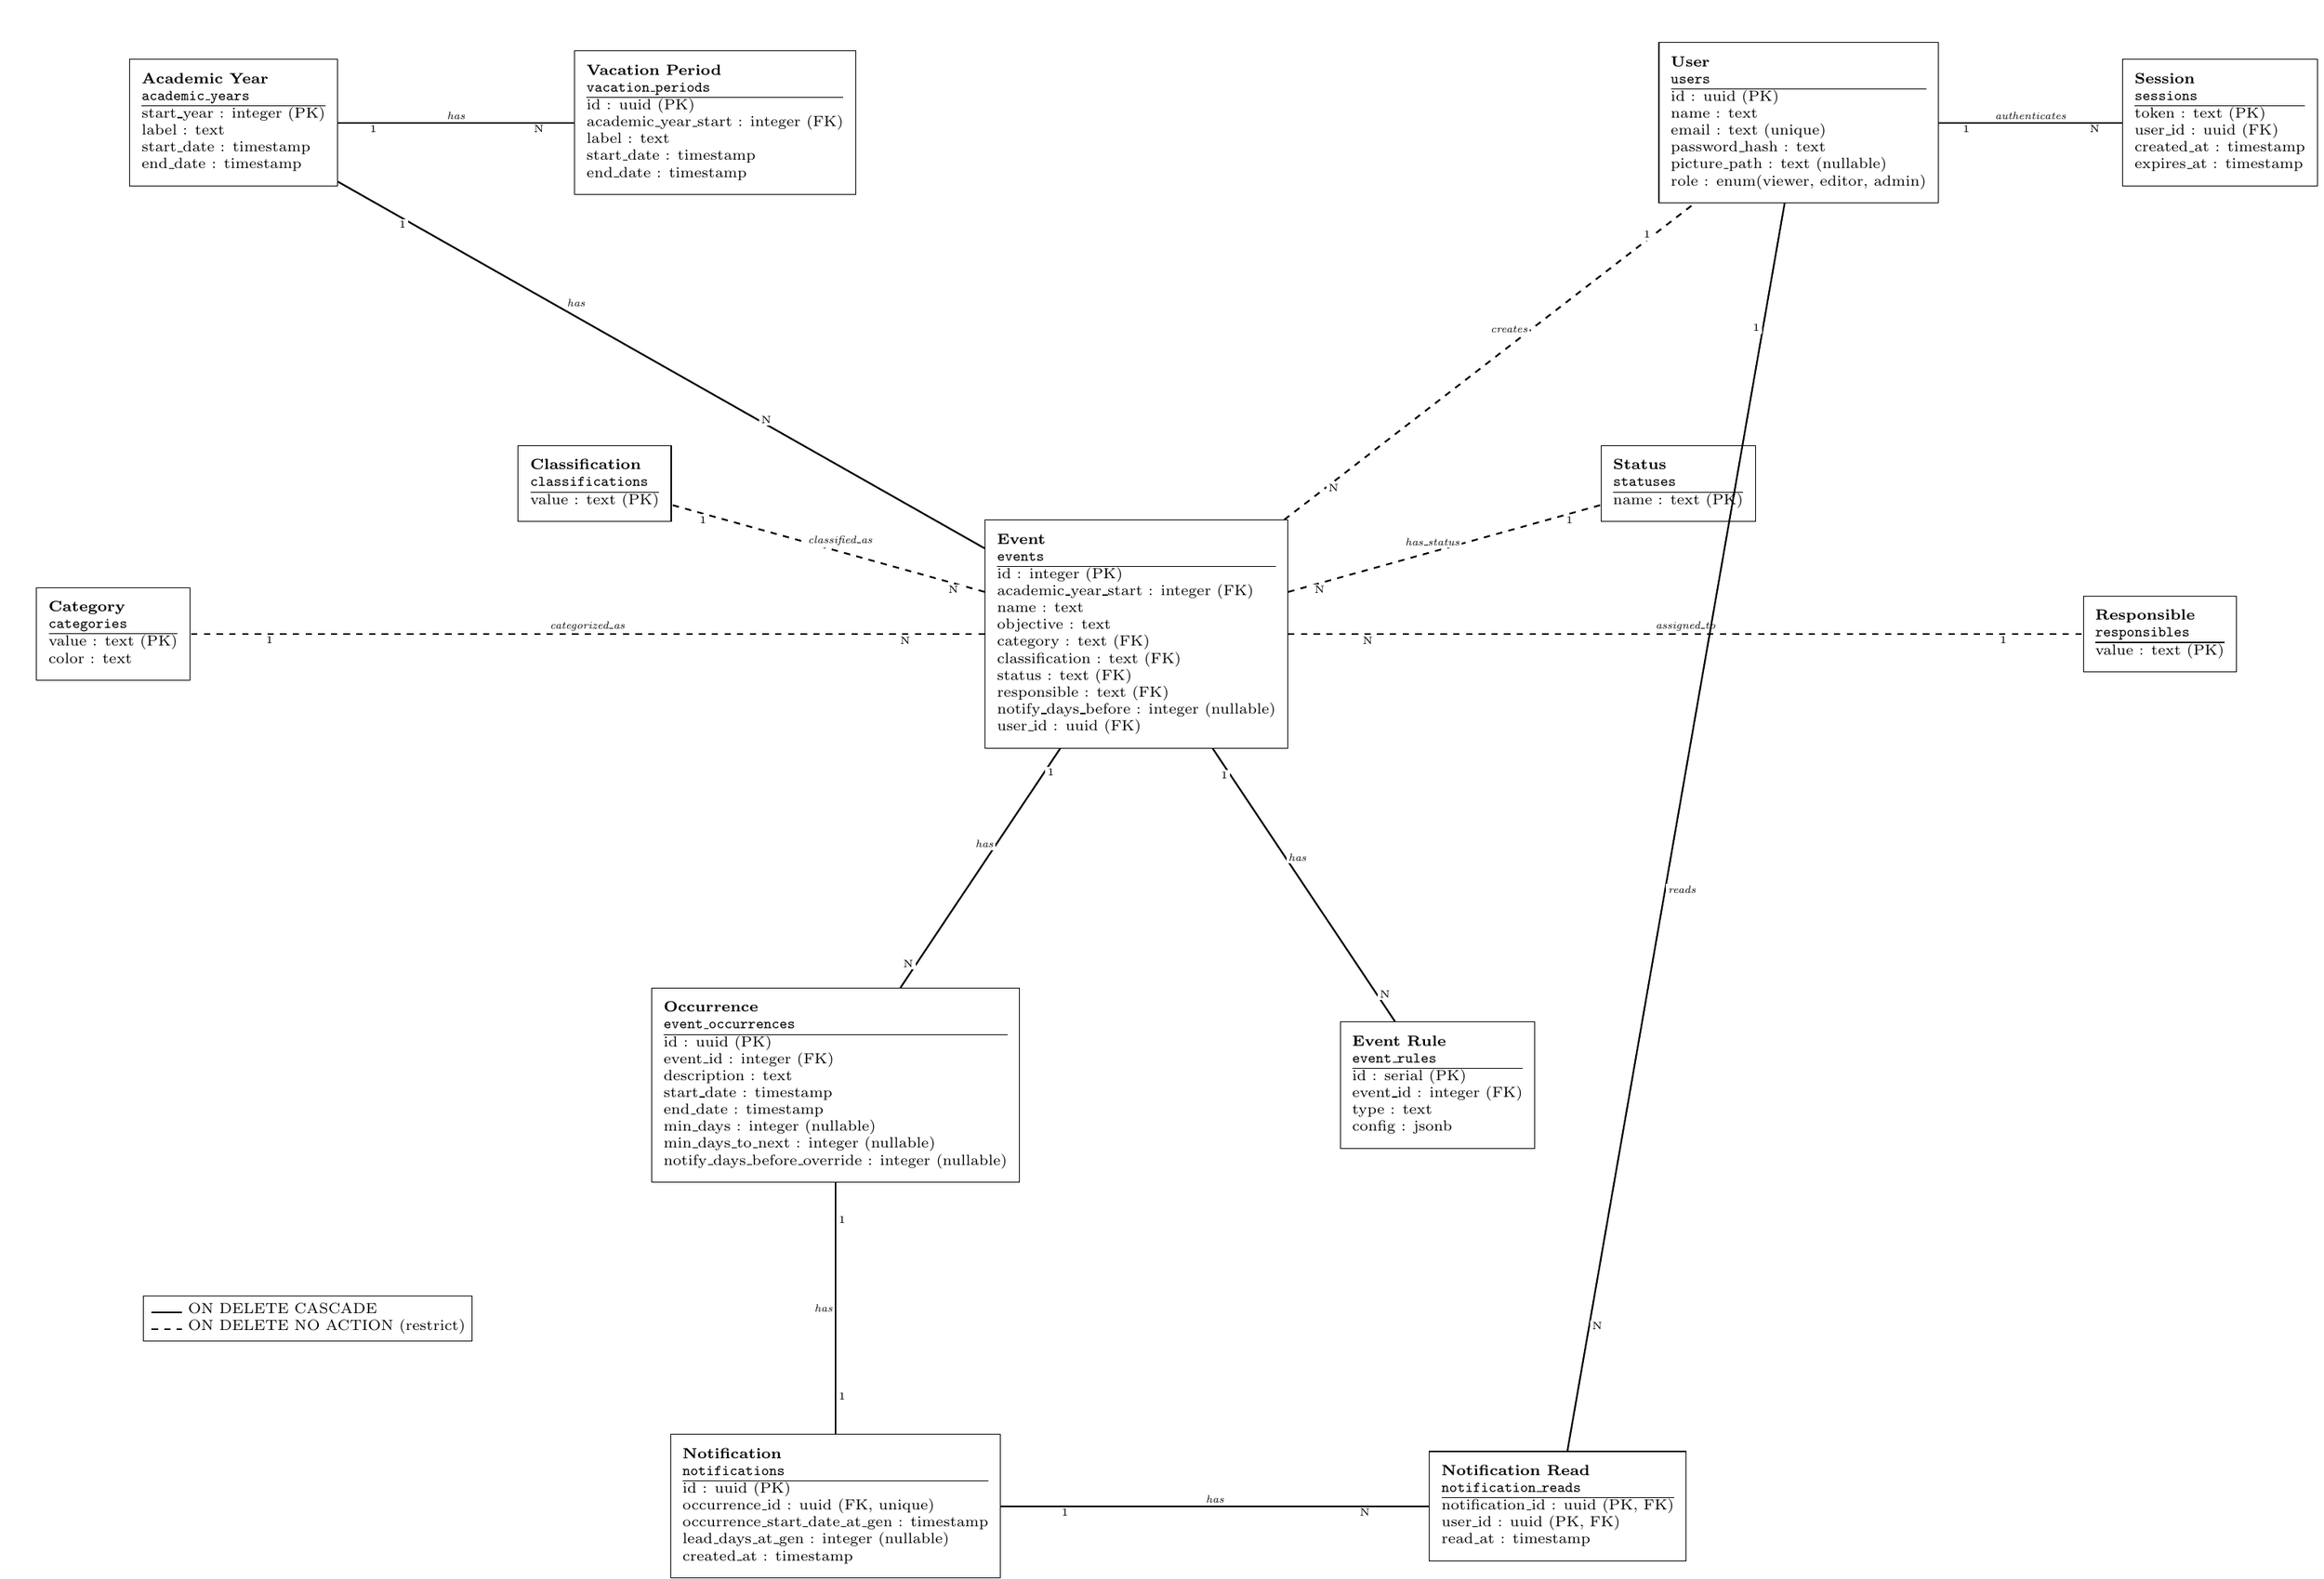
\begin{tikzpicture}[
    erentity/.style={draw, rectangle, align=left, font=\scriptsize, inner sep=2mm, fill=white},
    cascade/.style={thick},
    restrict/.style={thick, dashed},
    card/.style={fill=white, inner sep=1pt, font=\tiny},
    rel/.style={fill=white, inner sep=1pt, font=\tiny\itshape},
]

% --- entities, with full attribute lists ---
% Note: no three entities share both the same x and the same y-alignment as
% any drawn edge, so that no relationship line passes through an unrelated
% entity box (classifications/statuses are offset in y from the
% categories-event-responsibles spine for this reason).
\node[erentity] (academicyears) at (-15,9) {%
  \begin{tabular}{@{}l@{}}
    \textbf{Academic Year} \\ {\scriptsize\ttfamily academic\_years} \\ \hline
    start\_year : integer (PK) \\
    label : text \\
    start\_date : timestamp \\
    end\_date : timestamp
  \end{tabular}%
};

\node[erentity] (vacationperiods) at (-7,9) {%
  \begin{tabular}{@{}l@{}}
    \textbf{Vacation Period} \\ {\scriptsize\ttfamily vacation\_periods} \\ \hline
    id : uuid (PK) \\
    academic\_year\_start : integer (FK) \\
    label : text \\
    start\_date : timestamp \\
    end\_date : timestamp
  \end{tabular}%
};

\node[erentity] (users) at (11,9) {%
  \begin{tabular}{@{}l@{}}
    \textbf{User} \\ {\scriptsize\ttfamily users} \\ \hline
    id : uuid (PK) \\
    name : text \\
    email : text (unique) \\
    password\_hash : text \\
    picture\_path : text (nullable) \\
    role : enum(viewer, editor, admin)
  \end{tabular}%
};

\node[erentity] (sessions) at (18,9) {%
  \begin{tabular}{@{}l@{}}
    \textbf{Session} \\ {\scriptsize\ttfamily sessions} \\ \hline
    token : text (PK) \\
    user\_id : uuid (FK) \\
    created\_at : timestamp \\
    expires\_at : timestamp
  \end{tabular}%
};

\node[erentity] (categories) at (-17,0.5) {%
  \begin{tabular}{@{}l@{}}
    \textbf{Category} \\ {\scriptsize\ttfamily categories} \\ \hline
    value : text (PK) \\
    color : text
  \end{tabular}%
};

\node[erentity] (classifications) at (-9,3) {%
  \begin{tabular}{@{}l@{}}
    \textbf{Classification} \\ {\scriptsize\ttfamily classifications} \\ \hline
    value : text (PK)
  \end{tabular}%
};

\node[erentity] (event) at (0,0.5) {%
  \begin{tabular}{@{}l@{}}
    \textbf{Event} \\ {\scriptsize\ttfamily events} \\ \hline
    id : integer (PK) \\
    academic\_year\_start : integer (FK) \\
    name : text \\
    objective : text \\
    category : text (FK) \\
    classification : text (FK) \\
    status : text (FK) \\
    responsible : text (FK) \\
    notify\_days\_before : integer (nullable) \\
    user\_id : uuid (FK)
  \end{tabular}%
};

\node[erentity] (statuses) at (9,3) {%
  \begin{tabular}{@{}l@{}}
    \textbf{Status} \\ {\scriptsize\ttfamily statuses} \\ \hline
    name : text (PK)
  \end{tabular}%
};

\node[erentity] (responsibles) at (17,0.5) {%
  \begin{tabular}{@{}l@{}}
    \textbf{Responsible} \\ {\scriptsize\ttfamily responsibles} \\ \hline
    value : text (PK)
  \end{tabular}%
};

\node[erentity] (occurrences) at (-5,-7) {%
  \begin{tabular}{@{}l@{}}
    \textbf{Occurrence} \\ {\scriptsize\ttfamily event\_occurrences} \\ \hline
    id : uuid (PK) \\
    event\_id : integer (FK) \\
    description : text \\
    start\_date : timestamp \\
    end\_date : timestamp \\
    min\_days : integer (nullable) \\
    min\_days\_to\_next : integer (nullable) \\
    notify\_days\_before\_override : integer (nullable)
  \end{tabular}%
};

\node[erentity] (rules) at (5,-7) {%
  \begin{tabular}{@{}l@{}}
    \textbf{Event Rule} \\ {\scriptsize\ttfamily event\_rules} \\ \hline
    id : serial (PK) \\
    event\_id : integer (FK) \\
    type : text \\
    config : jsonb
  \end{tabular}%
};

\node[erentity] (notifications) at (-5,-14) {%
  \begin{tabular}{@{}l@{}}
    \textbf{Notification} \\ {\scriptsize\ttfamily notifications} \\ \hline
    id : uuid (PK) \\
    occurrence\_id : uuid (FK, unique) \\
    occurrence\_start\_date\_at\_gen : timestamp \\
    lead\_days\_at\_gen : integer (nullable) \\
    created\_at : timestamp
  \end{tabular}%
};

\node[erentity] (notificationreads) at (7,-14) {%
  \begin{tabular}{@{}l@{}}
    \textbf{Notification Read} \\ {\scriptsize\ttfamily notification\_reads} \\ \hline
    notification\_id : uuid (PK, FK) \\
    user\_id : uuid (PK, FK) \\
    read\_at : timestamp
  \end{tabular}%
};

% --- relationships ---
\draw[cascade] (academicyears) -- (vacationperiods) node[rel, midway, above] {has} node[card, pos=0.15, below] {1} node[card, pos=0.85, below] {N};
\draw[cascade] (academicyears) -- (event) node[rel, pos=0.35, above right] {has} node[card, pos=0.1, below] {1} node[card, pos=0.65, right] {N};

\draw[restrict] (event) -- (categories) node[rel, midway, above] {categorized\_as} node[card, pos=0.1, below] {N} node[card, pos=0.9, below] {1};
\draw[restrict] (event) -- (classifications) node[rel, midway, above, xshift=2mm] {classified\_as} node[card, pos=0.1, below] {N} node[card, pos=0.9, below] {1};
\draw[restrict] (event) -- (statuses) node[rel, midway, above, xshift=-2mm] {has\_status} node[card, pos=0.1, below] {N} node[card, pos=0.9, below] {1};
\draw[restrict] (event) -- (responsibles) node[rel, midway, above] {assigned\_to} node[card, pos=0.1, below] {N} node[card, pos=0.9, below] {1};

\draw[restrict] (event) -- (users) node[rel, pos=0.6, left] {creates} node[card, pos=0.1, right] {N} node[card, pos=0.9, left] {1};
\draw[cascade] (users) -- (sessions) node[rel, midway, above] {authenticates} node[card, pos=0.15, below] {1} node[card, pos=0.85, below] {N};

\draw[cascade] (event) -- (occurrences) node[rel, pos=0.4, left] {has} node[card, pos=0.1, right] {1} node[card, pos=0.9, left] {N};
\draw[cascade] (event) -- (rules) node[rel, pos=0.4, right] {has} node[card, pos=0.1, left] {1} node[card, pos=0.9, right] {N};

\draw[cascade] (occurrences) -- (notifications) node[rel, midway, left] {has} node[card, pos=0.15, right] {1} node[card, pos=0.85, right] {1};
\draw[cascade] (notifications) -- (notificationreads) node[rel, midway, above] {has} node[card, pos=0.15, below] {1} node[card, pos=0.85, below] {N};
\draw[cascade] (users) -- (notificationreads) node[rel, pos=0.55, right] {reads} node[card, pos=0.1, left] {1} node[card, pos=0.9, right] {N};

% --- legend ---
\node[draw, align=left, font=\scriptsize, anchor=north west, fill=white] at (-16.5,-10.5) {
    \tikz{\draw[cascade] (0,0) -- (0.5,0);} ON DELETE CASCADE \\
    \tikz{\draw[restrict] (0,0) -- (0.5,0);} ON DELETE NO ACTION (restrict)
};
\end{tikzpicture}%
}
\end{center}
\caption{Full Entity-Relationship Diagram with column-level attributes, derived from the Drizzle schema.}\label{fig:er-diagram-full}
\end{figure}
\end{landscape}

%
% Appendix B - Selected Code Listings
%
\chapter{Selected Code Listings} \label{app:code-listings}

This appendix gives the full, unabridged source of a few backend and frontend units that Chapters~\ref{cap:backend} and~\ref{cap:frontend} show only in an abbreviated form, to keep those chapters within the report's page budget.

\section{The Weekend Rule Definition} \label{app:weekend-rule}

Referenced from Section~\ref{sec:rule-engine}.

\begin{lstlisting}[caption={[The Weekend rule definition, in full.]{The Weekend rule definition, in full (\texttt{server/calendar/rules/definitions/weekend.rule.ts}).}}, label={lst:weekend-rule-full}]
export const weekendRule: IRuleDefinition = {
  id: "weekend",
  fields: [
    { id: "checkStart", type: "checkbox", defaultValue: true },
    { id: "checkEnd",   type: "checkbox", defaultValue: true },
    { id: "checkRange", type: "checkbox", defaultValue: false },
  ],
  translations: {
    pt: {
      label: "Fim de semana",
      fields: { checkStart: "Verificar início", checkEnd: "Verificar fim", checkRange: "Verificar período" },
      fieldLabels: { start: "Início", end: "Fim", range: "Período" },
      messages: {
        startIsWeekend: "O início coincide com um fim de semana",
        endIsWeekend: "O fim coincide com um fim de semana",
        rangeHasWeekend: "O período inclui um dia de fim de semana",
      },
    },
  },
  validate(_event, occurrence, config) {
    return runDayRangeCheck<true>({
      occurrence,
      config: config as WeekendConfig,
      matchDay: (day) => (isWeekend(day) ? true : undefined),
      toViolation: (field, date) => ({ fieldLabelKey: field, date, messageKey: MESSAGE_KEYS[field] }),
    });
  },
};
\end{lstlisting}

\clearpage
\section{The Global Rule-Validation Dispatcher} \label{app:collect-issues}

Referenced from Section~\ref{sec:rule-engine}.

\begin{lstlisting}[caption={[The global rule-validation dispatcher, in full.]{The global rule-validation dispatcher, in full (\texttt{server/calendar/services/calendar.service.ts}).}}, label={lst:collect-issues-full}]
private collectEventRuleIssues(
  event: IEvent,
  academicYearStart: number,
  allEvents: IEvent[],
  vacations: IVacationPeriod[] = [],
): ICalendarRuleIssue[] {
  const context = { allEvents, academicYearStart, vacations };
  const issues: ICalendarRuleIssue[] = [];

  const sortedOccurrences = [...event.occurrences].sort(
    (a, b) => new Date(a.startDate).getTime() - new Date(b.startDate).getTime(),
  );

  const pushIssues = (occurrence: (typeof sortedOccurrences)[number], ruleType: string, violations: IRuleViolation[]) => {
    for (const v of violations) {
      issues.push({
        eventId: event.id,
        eventName: event.name,
        occurrenceId: occurrence.id,
        occurrenceDescription: occurrence.description,
        academicYearStart,
        date: v.date,
        ruleType,
        fieldLabelKey: v.fieldLabelKey,
        messageKey: v.messageKey,
        messageParams: v.messageParams,
      });
    }
  };

  for (const occurrence of sortedOccurrences) {
    for (const builtInRule of [minDurationRule, minDaysToNextRule]) {
      pushIssues(occurrence, builtInRule.id, builtInRule.validate(event, occurrence, {}, context));
    }

    for (const rule of (event.rules ?? [])) {
      pushIssues(occurrence, rule.type, validateEventRule(rule, event, occurrence, context));
    }
  }

  return issues;
}
\end{lstlisting}

\clearpage
\section{Password Hashing and Verification} \label{app:crypto}

Referenced from Section~\ref{sec:backend-authentication}.

\begin{lstlisting}[caption={[Password hashing and verification, in full.]{Password hashing and verification, in full (\texttt{server/auth/crypto.ts}).}}, label={lst:crypto-full}]
export const hashPassword = (password: string): string => {
  const salt = crypto.randomBytes(16).toString("hex");
  const hash = crypto.scryptSync(password, salt, 64).toString("hex");
  return `scrypt$${salt}$${hash}`;
};

export const verifyPassword = (password: string, encodedHash: string): boolean => {
  const [algorithm, salt, storedHash] = encodedHash.split("$");
  if (algorithm !== "scrypt" || !salt || !storedHash) {
    return false;
  }

  const computedHash = crypto.scryptSync(password, salt, 64).toString("hex");
  if (computedHash.length !== storedHash.length) return false;
  return crypto.timingSafeEqual(
    Buffer.from(storedHash, "hex"),
    Buffer.from(computedHash, "hex"),
  );
};
\end{lstlisting}

\clearpage
\section{The withRolePolicy Authorization Wrapper} \label{app:with-role-policy}

Referenced from Section~\ref{sec:backend-rbac}.

\begin{lstlisting}[caption={[The withRolePolicy authorization wrapper, in full.]{The \texttt{withRolePolicy} authorization wrapper, in full (\texttt{server/shared/authorize.ts}).}}, label={lst:with-role-policy-full}]
export function withRolePolicy<
  TInstance extends object,
  TPolicy extends Partial<Record<keyof TInstance, TRolePolicy>>,
>(
  instance: TInstance,
  policy: TPolicy,
  getRole: (args: unknown[]) => TUserRole,
): { [K in keyof TPolicy]: TInstance[K & keyof TInstance] } {
  const wrapped: Record<string, unknown> = {};

  for (const key of Object.keys(policy)) {
    const minimum = policy[key as keyof TPolicy] as TRolePolicy;
    const original = instance[key as keyof TInstance] as unknown as
      (...args: unknown[]) => unknown;

    wrapped[key] = (...args: unknown[]) => {
      if (minimum !== "any") {
        assertRole(getRole(args), minimum);
      }
      return original.apply(instance, args);
    };
  }

  return wrapped as { [K in keyof TPolicy]: TInstance[K & keyof TInstance] };
}
\end{lstlisting}

\clearpage
\section{The DraggableEvent Component} \label{app:draggable-event}

Referenced from Section~\ref{sec:frontend-calendar-ui}.

\begin{lstlisting}[caption={[The DraggableEvent wrapper component, in full.]{The \texttt{DraggableEvent} wrapper component, in full (\texttt{features/calendar/dnd/draggable-event.tsx}).}}, label={lst:draggable-event-full}]
export function DraggableEvent({
  event,
  occurrence,
  children,
  className,
}: DraggableEventProps) {
  const { canEditEvents } = useCalendar();
  const { startDrag, endDrag, isDragging, draggedOccurrence } = useDragDrop();

  if (!canEditEvents) {
    return <>{children}</>;
  }

  const isCurrentlyDragged = isDragging && draggedOccurrence?.occurrence.id === occurrence.id;

  const handleClick = (e: React.MouseEvent<HTMLDivElement>) => {
    e.stopPropagation();
  };

  return (
    <motion.div
      className={`${className || ""} ${isCurrentlyDragged ? "opacity-50 cursor-grabbing" : "cursor-grab"}`}
      draggable
      onClick={(e: React.MouseEvent<HTMLDivElement>) => handleClick(e)}
      onDragStart={(e) => {
        (e as DragEvent).dataTransfer!.setData(
          "text/plain",
          occurrence.id,
        );
        startDrag(event, occurrence);
      }}
      onDragEnd={() => {
        endDrag();
      }}
    >
      {children}
    </motion.div>
  );
}
\end{lstlisting}

%
% Appendix C - Additional Screenshots
%
\chapter{Additional Screenshots} \label{app:screenshots}

This appendix gives full-size screenshots referenced from Chapter~\ref{cap:frontend} but not shown inline there, to keep that chapter within the report's page budget.

\section{Calendar Views} \label{app:calendar-views}

Referenced from Section~\ref{sec:frontend-calendar-ui}. The Month view is shown inline as Figure~\ref{fig:calendar}; the remaining four are given here in full size.

\begin{figure}[htbp]
\begin{center}
\resizebox{\textwidth}{!}{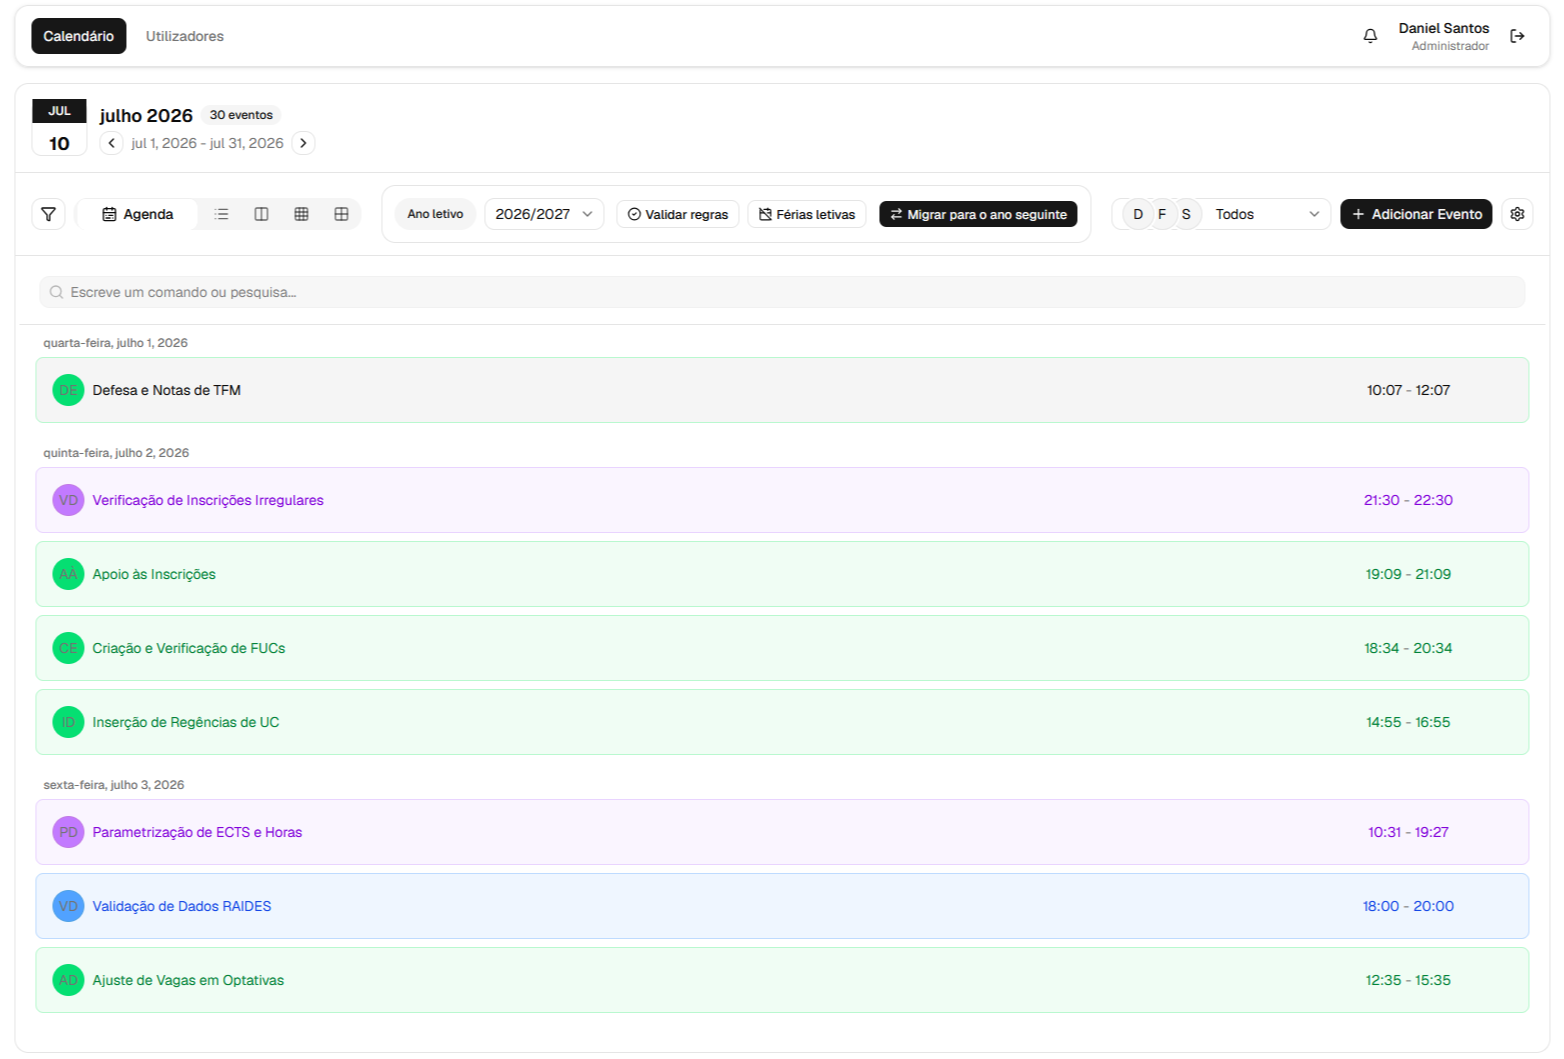
\includegraphics{./figures/app_screenshots/calendar_View_agenda.png}}
\end{center}
\caption{Calendar interface, Agenda view: a scrollable list of occurrences grouped by date or category.}\label{fig:calendar-agenda}
\end{figure}

\clearpage
\begin{figure}[htbp]
\begin{center}
\resizebox{\textwidth}{!}{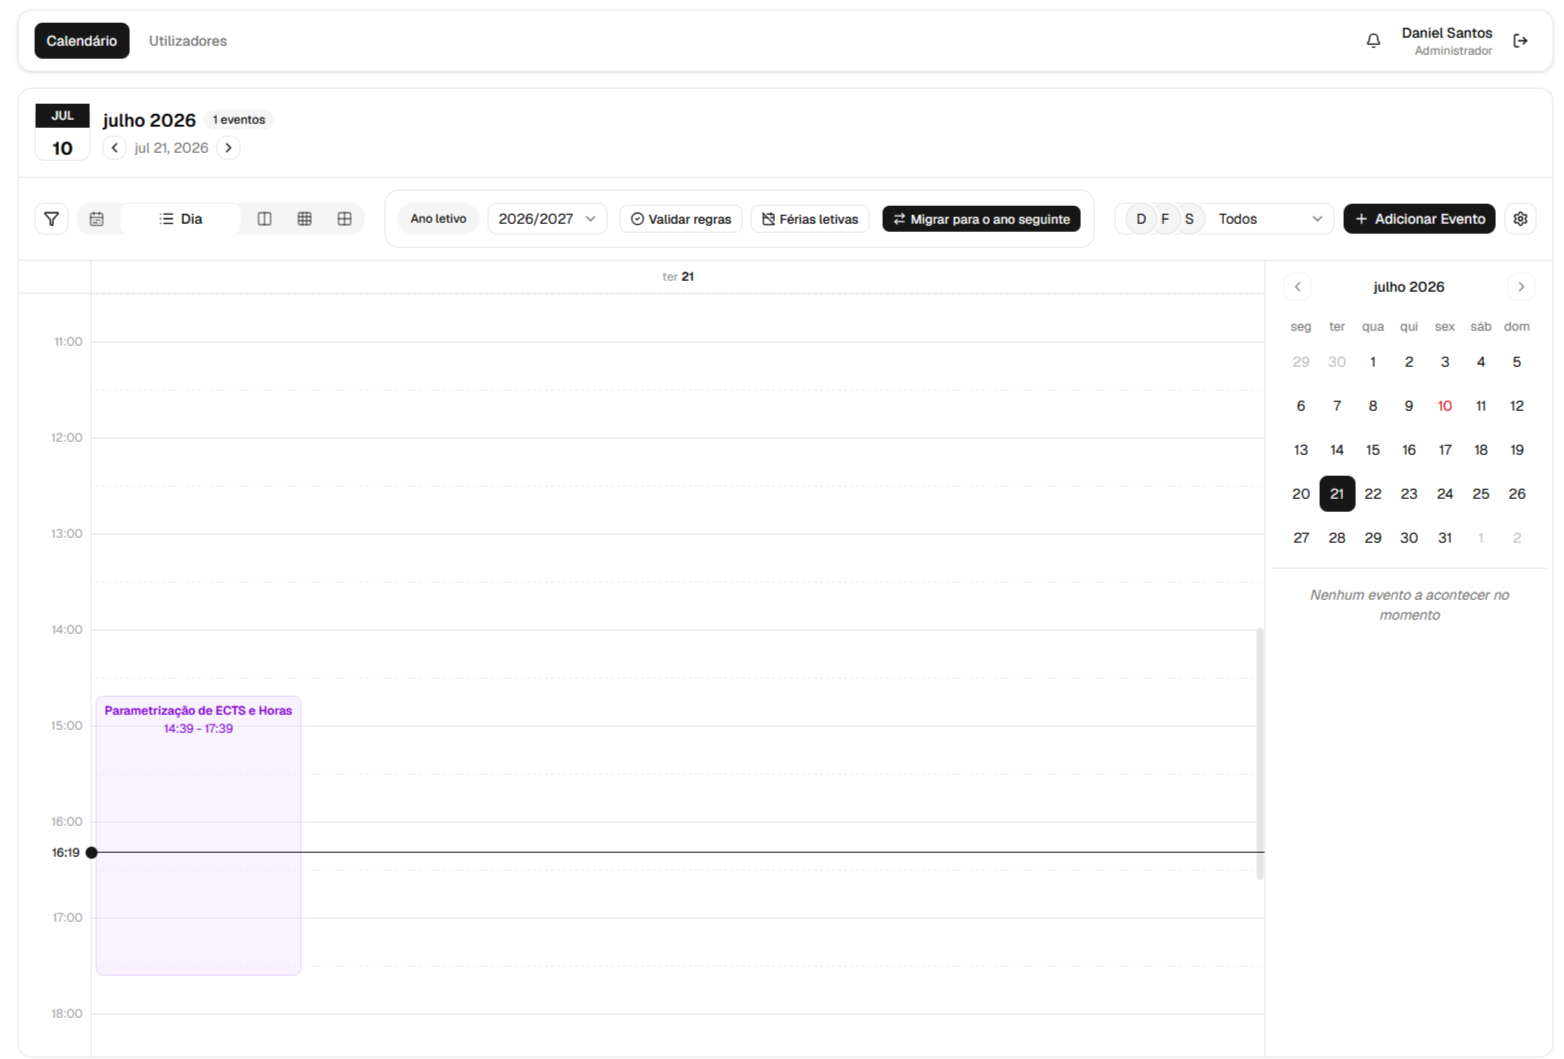
\includegraphics{./figures/app_screenshots/calendar_View_day.png}}
\end{center}
\caption{Calendar interface, Day view: a single-day time grid supporting drag-and-drop rescheduling and resizing.}\label{fig:calendar-day}
\end{figure}

\clearpage
\begin{figure}[htbp]
\begin{center}
\resizebox{\textwidth}{!}{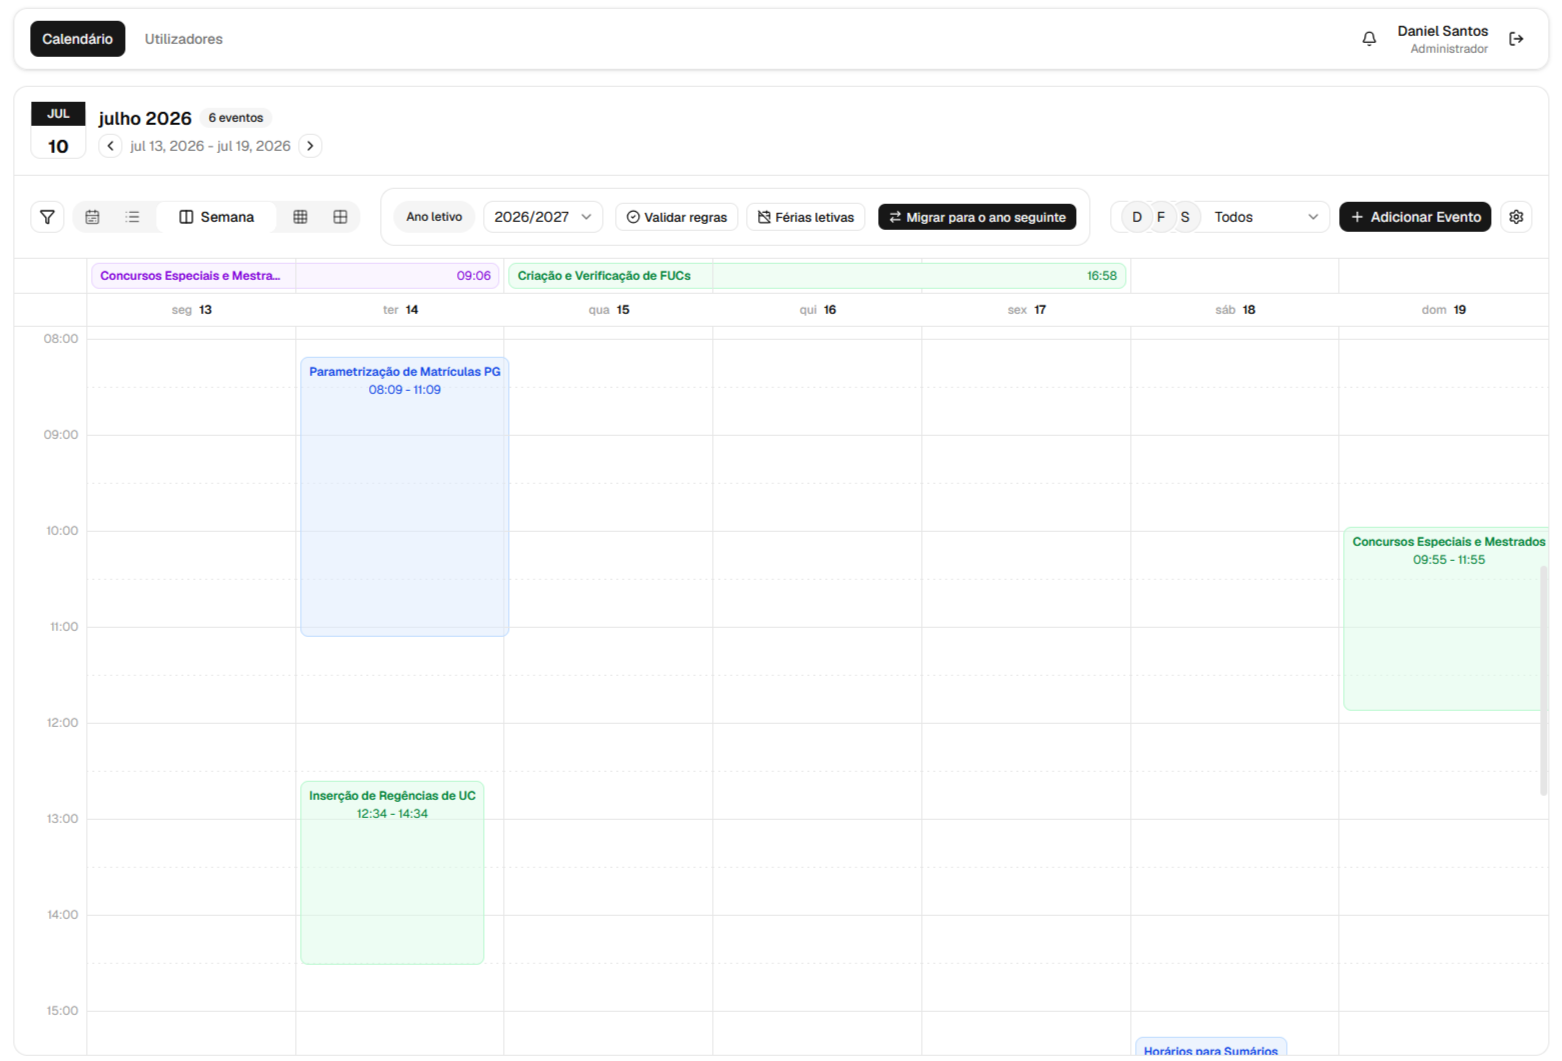
\includegraphics{./figures/app_screenshots/calendar_View_week.png}}
\end{center}
\caption{Calendar interface, Week view: the same time-grid interactions as the Day view, spanning a full week.}\label{fig:calendar-week}
\end{figure}

\clearpage
\begin{figure}[htbp]
\begin{center}
\resizebox{\textwidth}{!}{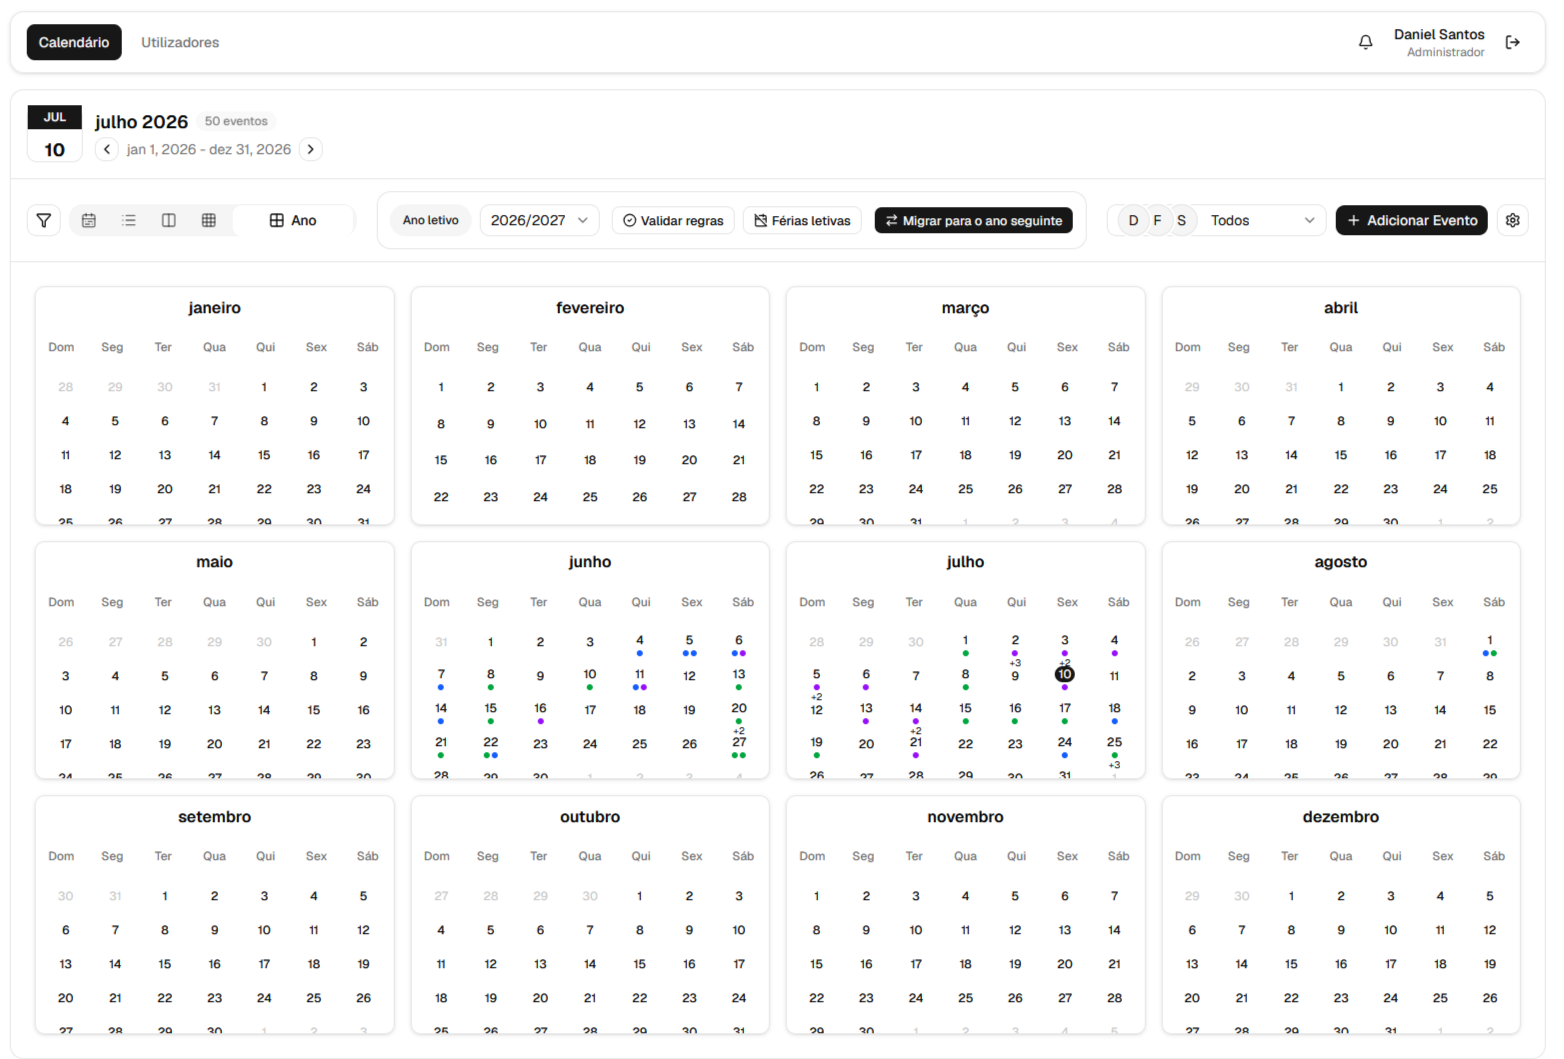
\includegraphics{./figures/app_screenshots/calendar_View_year.png}}
\end{center}
\caption{Calendar interface, Year view: a full-year grid overview of the academic calendar.}\label{fig:calendar-year}
\end{figure}

\clearpage
\section{Validation/Migration Results Modal} \label{app:migration-report}

Referenced from Section~\ref{sec:frontend-academic-year-tools}.

\begin{figure}[htbp]
\begin{center}
\resizebox{!}{160mm}{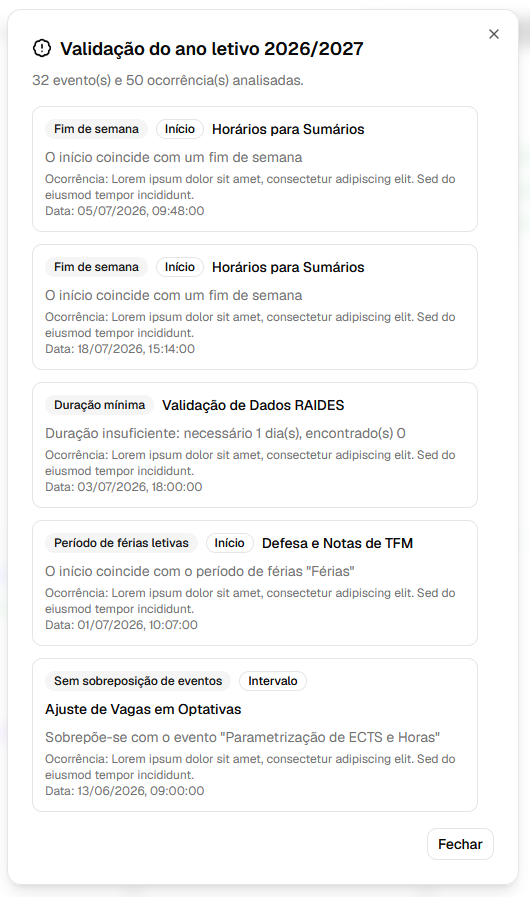
\includegraphics{./figures/app_screenshots/rules_validate.png}}
\end{center}
\caption{Validation/migration results modal: a confirmation banner when no rule violations are found, or one card per violation, each naming the rule, the affected event/occurrence, and the offending date.}\label{fig:migration-report-full}
\end{figure}


\end{document}